
\documentclass[xcolor={dvipsnames}]{beamer}
\usepackage{amsmath}
% \usepackage{beamerthemesplit} // Activate for custom appearance
\usepackage{hyperref}
\usepackage{ragged2e}
\usepackage{amssymb}
\usepackage{verbatim}
\usepackage{lmodern}
\input xy 
\xyoption{all}



\title{Neural Nets}
\author{Schwartz}
\date{\today}



\begin{document}

\frame{\titlepage}




{
\beamertemplatenavigationsymbolsempty
\frame{
 \frametitle{Making machines that think}
\vspace{-.75em}
{
\fontfamily{<familyname>}\selectfont
\begin{quote}
\tiny
\justify

$\;$The perceptron -- a single layer feedforward neural network -- was invented in 1957 at the Cornell Aeronautical Laboratory by Frank Rosenblatt with funding from the United States Office of Naval Research.
In a 1958 press conference organized by the US Navy, based on Rosenblatt's statements, The New York Times reported the perceptron to be ``the embryo of an electronic computer that [the Navy] expects will be able to walk, talk, see, write, reproduce itself and be conscious of its existence.''\\
\hspace{1.5em}Upon his death, the titular Reverend Thomas Bayes (1701--1761) of the renowned theorem left an unpublished manuscript deriving the distribution for the parameter of a binomial distribution. This found its way to Richard Price, who prior to posthumously reading the manuscript at the Royal Society, dutifully edited the manuscript and added an introduction that forms much of the philosophical basis for Bayesian analysis.  Mathematical historians have argued that ``by modern standards, we should refer to the Bayes-Price rule. Price discovered Bayes' work, recognized its importance, corrected it, contributed to the article, and found a use for it. The modern convention of employing Bayes' name alone is unfair but so entrenched that anything else makes little sense.'' Quite unaware of Bayes' work, the French mathematician Pierre-Simon Laplace reproduced and extended Bayes' results in 1774. It was also suggested that the blind English mathematician Nicholas Saunderson discovered the theorem some time before Bayes, but this is disputed.  \\
\hspace{1.5em}The elegant simplicity and effectiveness of Bayes' theorem for ``learning'' has prompted some psychologists to ask if the human brain itself might be a Bayesian-reasoning machine. They suggest that the Bayesian capacity to draw strong inferences from sparse data could be crucial to the way the mind perceives the world, plans actions, comprehends and learns language, reasons from correlation to causation, and even understands the goals and beliefs of other minds.  
The key to successful Bayesian reasoning is not in having an extensive, unbiased sample, which is the eternal worry of frequentists, but rather in having an appropriate ``prior''. This prior is an assumption about the way the world works. 
With the correct prior, even a single piece of data can be used to make meaningful Bayesian predictions. By contrast, 
frequentism is perhaps not well suited to making decisions on the basis of limited information -- which is something that people have to do all the time.  \\
\hspace{1.5em} It is thought by cognitive neuroscientists that neocortical development occurs in sequential layers, driven by waves of nerve growth factors which result in a self-organizating system. 
Modern so-called $\textrm{\emph{deep learning}}$ successors of the perceptron use
 Bayesian model fitting techniques to analogously sequentially train layer upon layer of neurons 
to produce \emph{unsupervised} (self-organizing) classification networks. 

%Researches have devised experiments to test if ``learning'' in the human brain copes with everyday judgments in the real world in a Bayesian manner. 

\end{quote}
}
}
}



\frame
{
\frametitle{Objectives}

f(a)=1/(1+e^-a)
g(a)=1+e^-a

d/da f(a) = d/dg dg/da f(g(a)) 

d/dg(a) f(g(a)) 
f = -1/(1+e^-a)^2

dg(a)/da = -e^-a 

product:
e^-a/(1+e^-a)^2
= e^-a/(1+e^-a)(1/(1+e^-a))
= (1 - 1/(1+e^-a)) (1/(1+e^-a))



\begin{itemize}
%\item understand image tools and pipelines
\item neural networks
\item activation functions
\item \textcolor{gray}{abstract feature encoding via layers}
\item \textcolor{gray}{neural networks $\Longrightarrow$ regression}
\item backpropegation (gradient decent via chain rule) 
\item[]
\item \textcolor{gray}{backpropegation parameter tuning}
\item \textcolor{gray}{images as data}
\item convolutions
\item convolutional networks
%\item understand there is new thing called deep learning\\
%that can be viewed as an extension of neural networks
\end{itemize}

}



\frame
{
 \frametitle{Artificial Neural Network (NN)}

\vspace{-1.62em}
\begin{columns}
\begin{column}{.6\textwidth}
\begin{itemize}
\item  \emph{NN's} are a collection of nodes $\eta^{(l)}_j$ that take on various states $\left\{\eta^{(l)}_j\right\}$
\item[]
\item[] \textcolor{white}{Features can be embedded into NNs as collections of states  }
\item[] \textcolor{white}{Nodes capture an idea or concept}
\item[] \textcolor{white}{These states can in turn be embedded in further layers of states}
\item[] \textcolor{white}{Each hierarchical layer provides higher orders of abstraction}
\item[]
\item[] \textcolor{white}{The transformation weights $w^{(l)}_{ij}$ and the topology provide the map from ``features'' to  ``states''}
\end{itemize}
\end{column}
\begin{column}{.5\textwidth}
\vspace{1.75em}

\xymatrix{
&& \\
& \left\{\eta^{(1)}_1\right\} &  \\
\textcolor{white}{X_{i1}}& \left\{\eta^{(1)}_2\right\}  & \\
& \left\{\eta^{(1)}_3\right\}  & \\
&& \\
}

\end{column}
\end{columns}

}



\frame
{
 \frametitle{Artificial Neural Network (NN)}
\begin{columns}
\begin{column}{.6\textwidth}
\begin{itemize}
\item  \emph{NN's} are a collection of nodes $\eta^{(l)}_j$ that take on various states $\left\{\eta^{(l)}_j\right\}$
\item<1-> Features are embedded into \\NNs as collections of states  
\end{itemize}
\footnotesize
\onslide<2->{
\begin{align*}
\text{via} \left\{\eta^{(1)}_1\right\} ={}& f\left(X^T{w^{(0)}_1}\right)\text{ where, e.g.} \\
%{\eta^{(2)}} ={}& f\left({W^{(0)}}^T{W^{(1)}}^TX\right)\\
X_i ={}& \left( X_{i1}, X_{i2}, X_{i3} \right)^T \\
%{\eta^{(1)}} ={}& \left[ \eta^{(1)}_1, \eta^{(1)}_2, \eta^{(1)}_3 \right]^T\\
%{\eta^{(1)}} ={}& \left[ \eta^{(1)}_1, \eta^{(1)}_2, \eta^{(1)}_3, \eta^{(1)}_4, \eta^{(1)}_5 \right]^T\\
w^{(0)}_j ={}& \left(w^{{(0)}_{1j}}, w^{{(0)}_{2j}}, w^{{(0)}_{3j}}\right)^T \\
\text{with }& \text{activation function $f$}
%W^{(1)} ={}& \left[\begin{array}{ccc} w^{{(0)}_{11}} & w^{{(0)}_{12}} & w^{{(0)}_{13}} \\ w^{{(0)}_{21}} & w^{{(0)}_{22}} & w^{{(0)}_{23}} \\ w^{{(0)}_{31}} & w^{{(0)}_{32}} & w^{{(0)}_{33}} \\ \end{array}\right]
%\text{etc.}
\end{align*}}

\vspace{-2.5em}
\begin{itemize}
\item<2>[]
\fbox{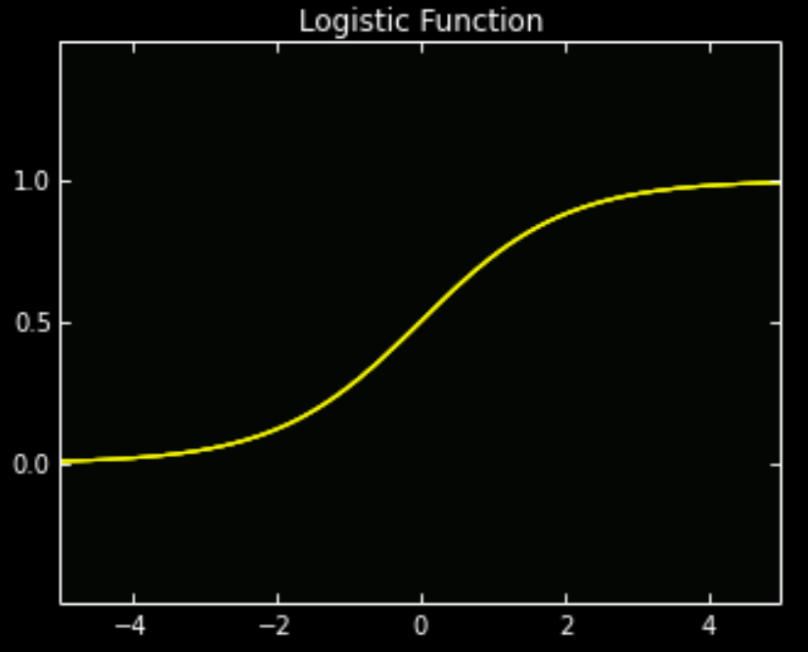
\includegraphics[width=2in,height=1.35in]{stuff/activationf2.png}}
\vspace{-1.515in}
\item<3>[]
\fbox{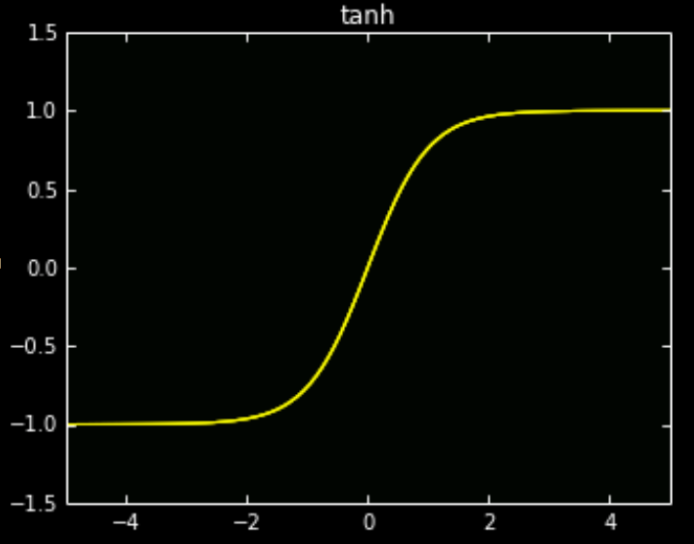
\includegraphics[width=2in,height=1.35in]{stuff/activationf4.png}}
\vspace{-1.515in}
\item<4>[]
\fbox{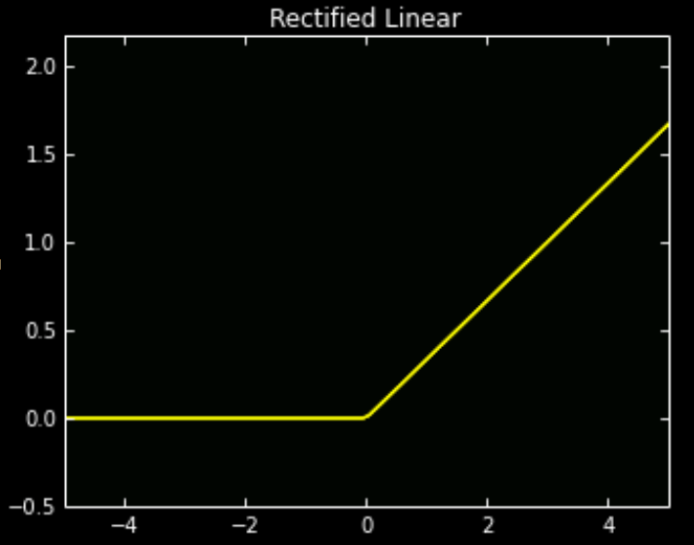
\includegraphics[width=2in,height=1.35in]{stuff/activationf3.png}}
\vspace{-1.515in}
\item<5>[]
\fbox{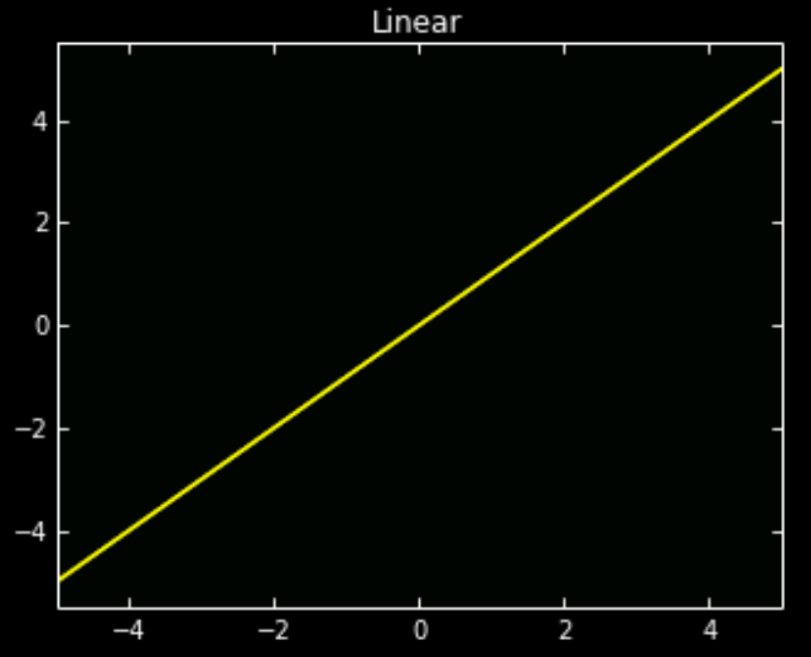
\includegraphics[width=2in,height=1.35in]{stuff/activationf1.png}}
\end{itemize}


\end{column}
\begin{column}{.5\textwidth}
\xymatrix{
&&  \\
X_{i1} \ar[dr]|{w^{{(0)}_{12}}} \ar[ddr]|>>>>>>{w^{{(0)}_{13}}} \ar[r]^{w^{{(0)}_{11}}}  & \left\{\eta^{(1)}_1\right\}   &  \\
X_{i2} \ar@{.}[r] \ar@{.}[dr] \ar@{.}[ur] & \left\{\eta^{(1)}_2\right\} &\\
X_{i3} \ar@{.}[ur] \ar@{.}[uur] \ar@{.}[r] & \left\{\eta^{(1)}_3\right\}  &\\
&& \\
}

\end{column}
\end{columns}

}




\frame
{
 \frametitle{Artificial Neural Network (NN)}
\begin{columns}
\begin{column}{.6\textwidth}
\begin{itemize}
\item  \emph{NN's} are a collection of nodes $\eta^{(l)}_j$ that take on various states $\left\{\eta^{(l)}_j\right\}$
\item<1-> Features are embedded into \\NNs as collections of states  
\end{itemize}
\footnotesize
\onslide<1->{
\begin{align*}
\text{via} \left\{\eta^{(1)}_1\right\} ={}& f\left(X^T{w^{(0)}_1}\right)\text{ where, e.g.} \\
%{\eta^{(2)}} ={}& f\left({W^{(0)}}^T{W^{(1)}}^TX\right)\\
X_i ={}& \left( X_{i1}, X_{i2}, X_{i3} \right)^T \\
%{\eta^{(1)}} ={}& \left[ \eta^{(1)}_1, \eta^{(1)}_2, \eta^{(1)}_3 \right]^T\\
%{\eta^{(1)}} ={}& \left[ \eta^{(1)}_1, \eta^{(1)}_2, \eta^{(1)}_3, \eta^{(1)}_4, \eta^{(1)}_5 \right]^T\\
w^{(0)}_j ={}& \left(w^{{(0)}_{1j}}, w^{{(0)}_{2j}}, w^{{(0)}_{3j}}\right)^T \\
\text{with }& \text{activation function $f$}
%W^{(1)} ={}& \left[\begin{array}{ccc} w^{{(0)}_{11}} & w^{{(0)}_{12}} & w^{{(0)}_{13}} \\ w^{{(0)}_{21}} & w^{{(0)}_{22}} & w^{{(0)}_{23}} \\ w^{{(0)}_{31}} & w^{{(0)}_{32}} & w^{{(0)}_{33}} \\ \end{array}\right]
%\text{etc.}
\end{align*}}

\vspace{-2.5em}
\begin{itemize}
\item<1>[]
\fbox{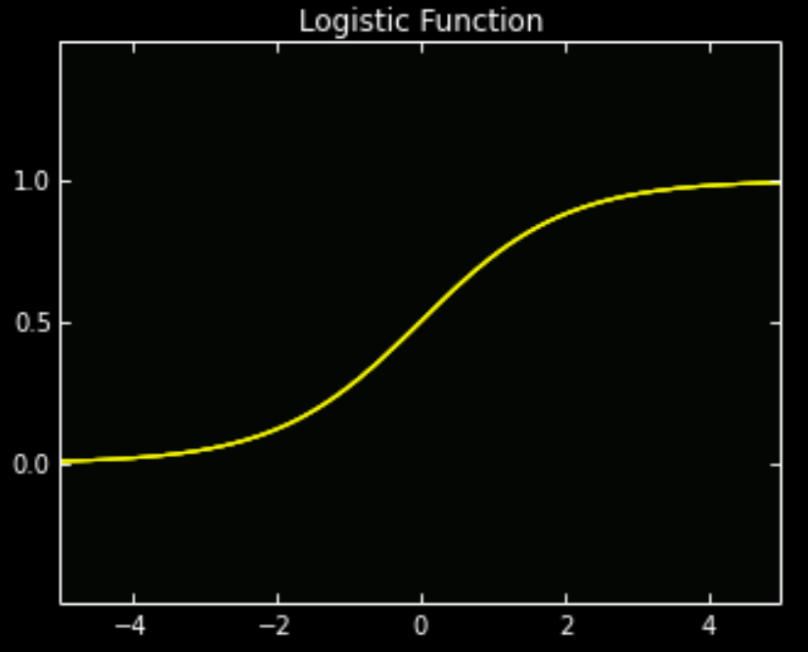
\includegraphics[width=2in,height=1.35in]{stuff/activationf2.png}}
\vspace{-1.515in}
\item<2>[]
\fbox{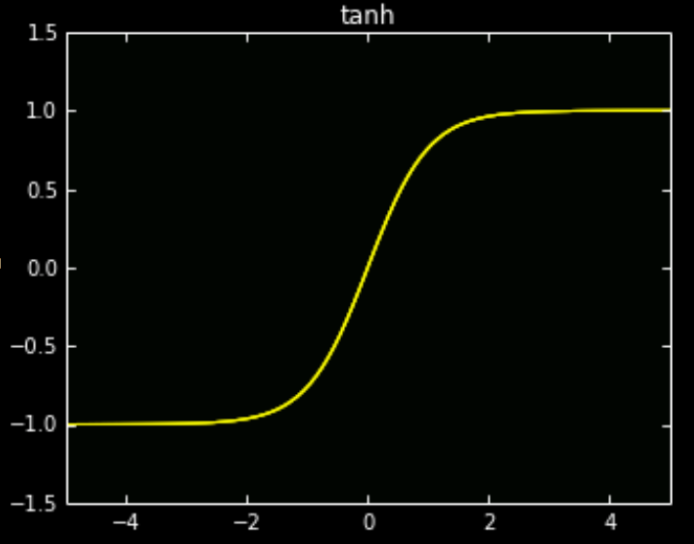
\includegraphics[width=2in,height=1.35in]{stuff/activationf4.png}}
\vspace{-1.515in}
\item<3>[]
\fbox{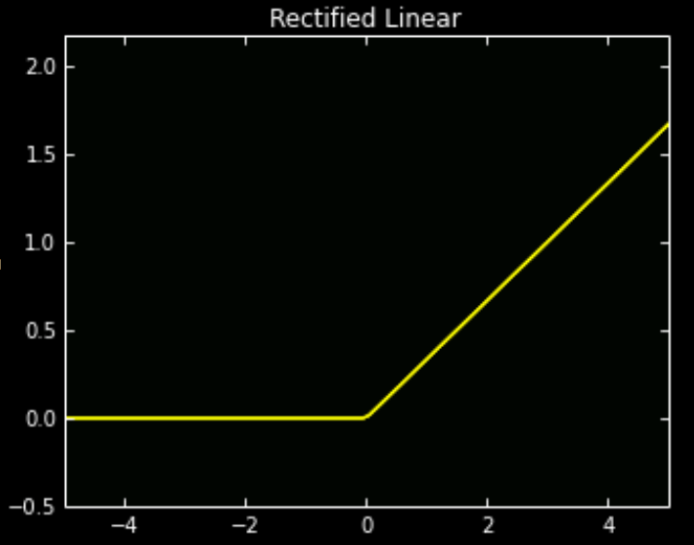
\includegraphics[width=2in,height=1.35in]{stuff/activationf3.png}}
\vspace{-1.515in}
\item<4>[]
\fbox{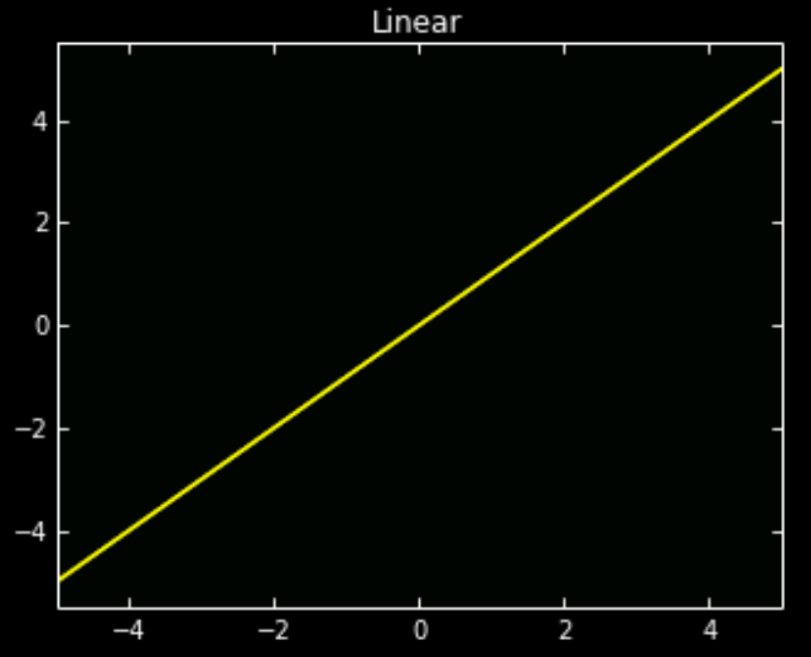
\includegraphics[width=2in,height=1.35in]{stuff/activationf1.png}}
\end{itemize}


\end{column}
\begin{column}{.5\textwidth}


\vspace{-.35em}

\xymatrix{
&&  \\
X_{i1} \ar[dr]|{w^{{(0)}_{12}}} \ar[ddr]|>>>>>>{w^{{(0)}_{13}}} \ar[r]^{w^{{(0)}_{11}}}  & \left\{\eta^{(1)}_1\right\}   &  \\
X_{i2} \ar@{.}[r] \ar@{.}[dr] \ar@{.}[ur] & \left\{\eta^{(1)}_2\right\} &\\
X_{i3} \ar@{.}[ur] \ar@{.}[uur] \ar@{.}[r] & \left\{\eta^{(1)}_3\right\}  &\\
&& \\
}

\vspace{-1.5em}


\textcolor{Maroon}{
\emph{\underline{Action potentials} fire when a \\ neuron (node) is turned ``on''}}


\end{column}
\end{columns}

}



\frame
{
\frametitle{Artificial Neural Network (NN) \textcolor{gray}{[thoughts?]}}

\begin{columns}
\begin{column}{.6\textwidth}
\begin{itemize}
\item  \emph{NN's} are a collection of nodes $\eta^{(l)}_j$ that take on various states $\left\{\eta^{(l)}_j\right\}$
\item Features are embedded into\\ NNs as collections of states  
\item<1->[] \textcolor{Maroon}{\emph{capturing an ``idea'' or ``concept''}}
\item[] \textcolor{White}{
\emph{\underline{Action potentials} fire when a \\ neuron (node) is turned ``on''}}
\item[]
\item[]
\item[]
\item[]
\item[]
\item[]
\item[]
\item[]
\item[]
\end{itemize}
\end{column}
\begin{column}{.5\textwidth}

\vspace{-2em}

\xymatrix{
&&  \\
X_{i1} \ar[dr]|{w^{{(0)}_{12}}} \ar[ddr]|>>>>>>{w^{{(0)}_{13}}} \ar[r]^{w^{{(0)}_{11}}}  & \left\{\eta^{(1)}_1\right\}   &  \\
X_{i2} \ar@{.}[r] \ar@{.}[dr] \ar@{.}[ur] & \left\{\eta^{(1)}_2\right\} &\\
X_{i3} \ar@{.}[ur] \ar@{.}[uur] \ar@{.}[r] & \left\{\eta^{(1)}_3\right\}  &\\
&& \\
}

\vspace{.25em}
\end{column}
\end{columns}

}



\frame
{
 \frametitle{Artificial Neural Network (NN) \textcolor{black}{[thoughts?]}}

\begin{columns}
\begin{column}{.6\textwidth}
\begin{itemize}
\item  \emph{NN's} are a collection of nodes $\eta^{(l)}_j$ that take on various states $\left\{\eta^{(l)}_j\right\}$
\item Features are embedded into\\ NNs as collections of states  
\item[] \textcolor{Maroon}{\emph{capturing an ``idea'' or ``concept''}}
\item These can be further combined\\ in subsequent layers of states
\item[]<2-> \textcolor{NavyBlue}{\emph{Each hierarchical layer provides higher orders of abstraction}}
\item<3-> An NN's state at any time is it's current representation of data...
%\vspace{-.5in}\hspace{2in}What are the \\``thoughts'' of a NN?
\item[]
\item<4->[] \emph{Similar states for ``similar'' \\$X_i$'s means the NN \underline{knows}, or understands or ``recognizes'' $X_i$} 
\item[] 
\end{itemize}
\end{column}
\begin{column}{.5\textwidth}
\xymatrix{
&&  \left\{\eta^{(2)}_1\right\}\\
X_{i1} \ar[dr]|{w^{{(0)}_{12}}} \ar[ddr]|>>>>>>{w^{{(0)}_{13}}} \ar[r]^{w^{{(0)}_{11}}}  & \left\{\eta^{(1)}_1\right\} \ar[ur]|{w^{{(1)}_{11}}} \ar[dr]|<<<<<<{w^{{(1)}_{13}}} \ar[ddr]|>>>>>>{w^{{(1)}_{14}}} \ar[dddr]|>>>>>>{w^{{(1)}_{15}}}  \ar[r]^{w^{{(1)}_{12}}}  & \left\{\eta^{(2)}_2\right\}  \\
X_{i2} \ar@{.}[r] \ar@{.}[dr] \ar@{.}[ur] & \left\{\eta^{(1)}_2\right\}  \ar@{.}[r] \ar@{.}[dr] \ar@{.}[ur]  \ar@{.}[ddr] \ar@{.}[uur]  &\left\{\eta^{(2)}_3\right\} \\
X_{i3} \ar@{.}[ur] \ar@{.}[uur] \ar@{.}[r] & \left\{\eta^{(1)}_3\right\}  \ar@{.}[r] \ar@{.}[dr] \ar@{.}[ur]  \ar@{.}[uuur] \ar@{.}[uur]  &\left\{\eta^{(2)}_4\right\}\\
&&  \left\{\eta^{(2)}_5\right\}\\
}
\vspace{.25em}
\end{column}
\end{columns}


}



\frame
{
 \frametitle{Softmax}

\vspace{-2em}

\begin{columns}
\begin{column}{.15\textwidth}
\end{column}
\begin{column}{.35\textwidth}

\xymatrix{
&&  \eta_1 \\
X_{i1} \ar[dr]|{w^{{(0)}_{12}}} \ar[ddr]|>>>>>>{w^{{(0)}_{13}}} \ar[r]^{w^{{(0)}_{11}}}  & \left\{\eta^{(1)}_1\right\} \ar[ur]|{w^{{(1)}_{11}}} \ar[dr]|<<<<<<{w^{{(1)}_{13}}} \ar[ddr]|>>>>>>{w^{{(1)}_{14}}} \ar[dddr]|>>>>>>{w^{{(1)}_{15}}}  \ar[r]^{w^{{(1)}_{12}}}  &  \eta_2   \\
X_{i2} \ar@{.}[r] \ar@{.}[dr] \ar@{.}[ur] & \left\{\eta^{(1)}_2\right\}  \ar@{.}[r] \ar@{.}[dr] \ar@{.}[ur]  \ar@{.}[ddr] \ar@{.}[uur]  & \eta_3  \\
X_{i3} \ar@{.}[ur] \ar@{.}[uur] \ar@{.}[r] & \left\{\eta^{(1)}_3\right\}  \ar@{.}[r] \ar@{.}[dr] \ar@{.}[ur]  \ar@{.}[uuur] \ar@{.}[uur]  & \eta_4\\
&&  \eta_5 \\
}

\end{column}
\begin{column}{.6\textwidth}

\begin{figure}
\centering
Choose the class with\\ the largest probability 
\end{figure}
$$\displaystyle {exp(\eta_k)}/{\sum^K_{k'=1} exp(\eta_{k'})} $$

\begin{figure}
\centering
Define a loss function \\ on those predictions \\ ${}$\\ And Optimize!
\end{figure}

\end{column}
\end{columns}

\vspace{1em}

\onslide<2->{
\textcolor{NavyBlue}{Numerically similar inputs of course invoke similar states}

\textcolor{Maroon}{But really what we want is the same output states for "similar" input "things" -- i.e., inputs that should have the same outputs!}
}
}


\frame
{
 \frametitle{``Similar'' $X$'s that aren't that \emph{similar}... }

\begin{figure}
\centering
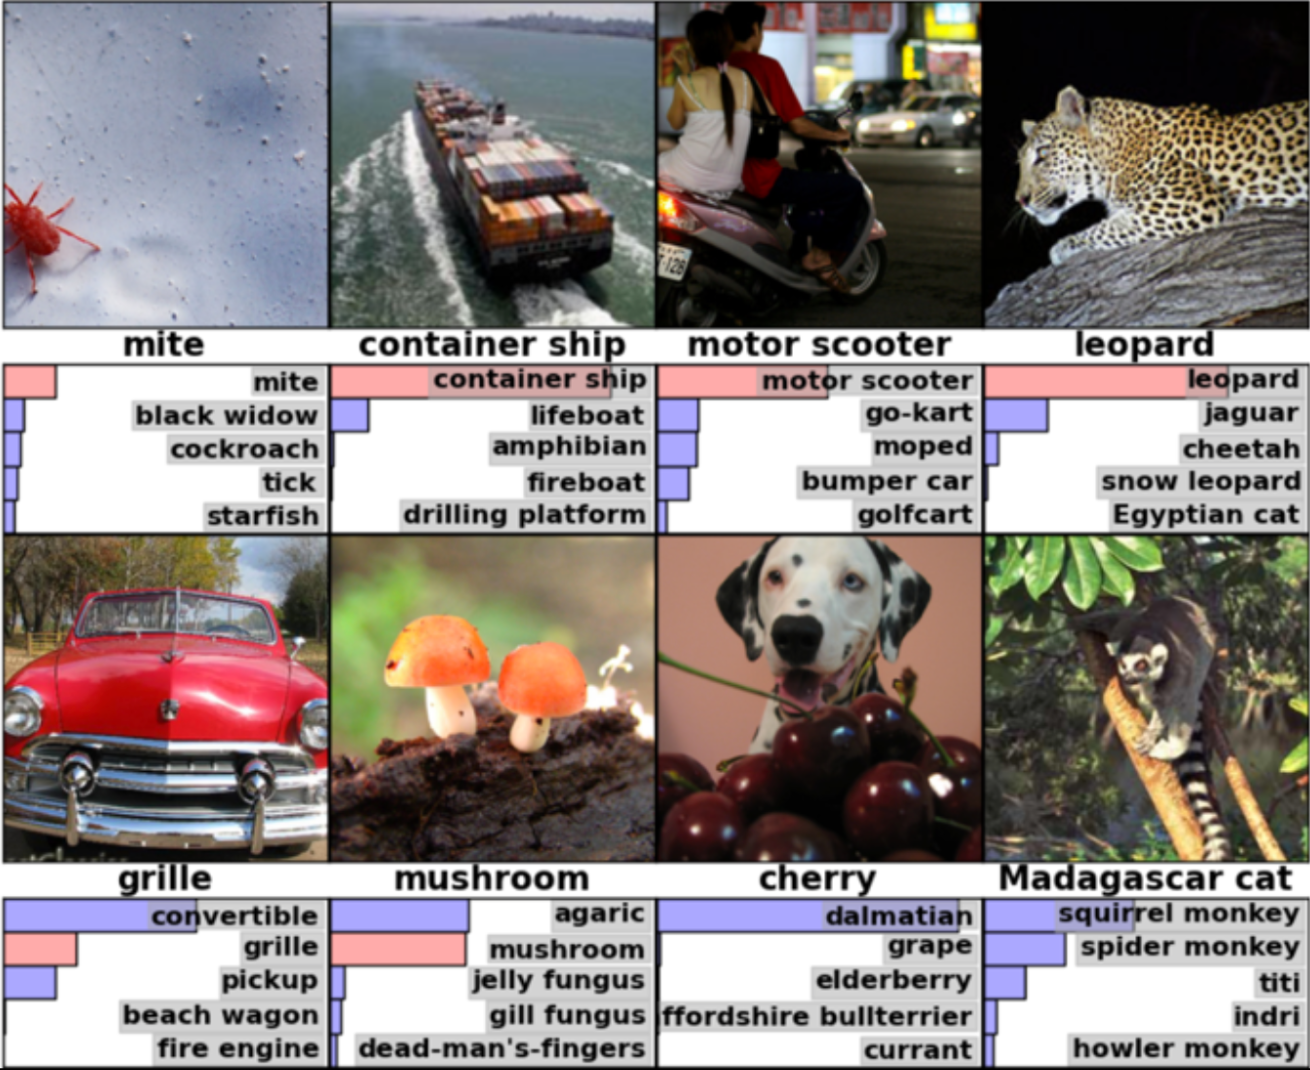
\includegraphics[width=3.8in]{stuff/pattern_rec.png}
\end{figure}

}



\frame
{
 \frametitle{Using NN's: where the fun ends and the pain begins}

\begin{itemize}
\item So patterns are trained (embedded) into an NN...
\item<2-> \underline{We have to specify the topology}

\vspace{1em}
\hspace*{-2.5em}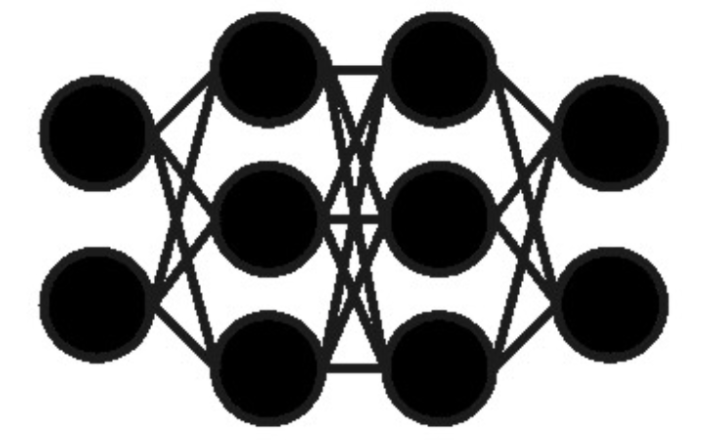
\includegraphics[height=.9in]{stuff/topologyC.png}$\quad$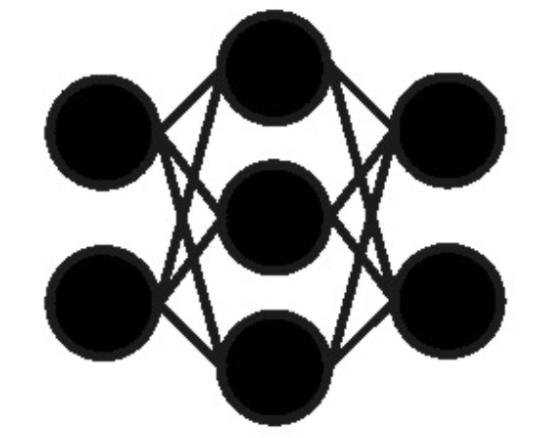
\includegraphics[height=.9in]{stuff/topologyA.png}$\quad$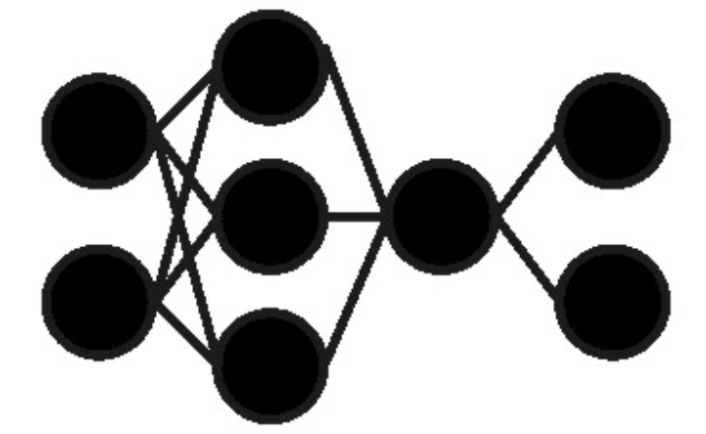
\includegraphics[height=.9in]{stuff/topologyB.png}

\hspace*{.25em}
\item<3-> Training patterns into a \emph{Deep NN (DNN)} is challenging...
\item<4->[] Let's start simple...
\end{itemize}
}


\frame
{
 \frametitle{Example NNs (Regression and Logistic Regression)}

%We'll train the NN with a squared loss cost function $\frac{1}{2}\sum(Y_i-\hat Y_i)^2$\\${}$\\

\begin{columns}
\begin{column}{.5\textwidth}
\hspace{.4in}
\xymatrix{
1 \ar[r]|{\beta_0}& \overset{\textcolor{gray}{(\hat Y)}}{\left\{ \eta \right\}} \\
X \ar[ur]|{\beta_1} &  }
\end{column}
\begin{column}{.5\textwidth}
%\hspace{1.75in}
\xymatrix{
1 \ar[r]|{\beta_0}&\overset{\textcolor{gray}{(\hat p)}}{\left\{ \eta \right\}}   \\
X \ar[ur]|{\beta_1} & }
\end{column}
\end{columns}

\footnotesize
\begin{columns}
\begin{column}{.5\textwidth}
\vspace{-.125in}
\begin{align*}
\hat Y = {}&  f\left( [1,x] \left[\begin{array}{c}\beta_0\\\beta_1\end{array}\right] \right) \\
= {}& [1,x] \left[\begin{array}{c}\beta_0\\\beta_1\end{array}\right]  = \beta_0 + \beta_1x\\{}\\
{}& \underset{\hat Y}{\text{min}} \frac{1}{2}\sum(Y_i-\hat Y_i)^2\\{}\\
\hat \beta ={}& \underset{\beta}{\text{argmin}} \frac{1}{2}\sum(Y_i-\beta_0 + \beta_1x_i)^2\\
\end{align*}
\end{column}
\begin{column}{.5\textwidth}
\begin{align*}
\hat p = {}&  f\left( [1,x] \left[\begin{array}{c}\beta_0\\\beta_1\end{array}\right] \right) \\
= {}& \frac{1}{1+e^{-(\beta_0 + \beta_1x)}} \textcolor{white}{\left[\begin{array}{c}\beta_0\\\beta_1\end{array}\right]}\\{}\\
{}& \underset{{\boldsymbol p}}{\text{min}} -\prod Y_i \log(p_i) + (1- Y_i)\log(1-p_i)\\{}\\
\hat \beta ={}& \underset{\beta}{\text{argmin}}  -\prod Y_i \log\left(\frac{1}{1+e^{-(\beta_0 + \beta_1x_i)}}\right) \\
{}&\quad\quad\quad\quad\quad\;\;+ (1- Y_i)\log\left(\frac{1}{1+e^{\beta_0 + \beta_1x_i}}\right) 
\end{align*}
\end{column}
\end{columns}

%${}$\\${}$\\
%\onslide<2->{Oh my doesn't that look familiar...} \onslide<3->{okay let's try again}


% We'll train the NN using the log loss cost function, $-\log L(\hat {\boldsymbol Y}|{\boldsymbol Y})$\\${}$\\

%${}$\\${}$\\
%\onslide<2->{Oh... we've also already done that...} \onslide<3->{okay, what gives}
}



\frame
{
 \frametitle{Forward propagation \textcolor{gray}{[And how to update parameters?]}}
 
$$\hat Y = \Huge f \tiny \left( \Huge f \tiny \left(\underset{n \times 3}{\left[\begin{array}{ccc} x_{11} & x_{12} & x_{13}\\x_{21} & x_{22} & x_{23}\\ \vdots&\vdots&\vdots\\x_{n1} & x_{n2} & x_{n3}\\ \end{array} \right]} \cdot  \underset{3 \times p}{\left[\begin{array}{cccc} w^0_{11} & w^0_{12} &\cdots &w^0_{1p}\\w^0_{21} & w^0_{22} &\cdots &w^0_{2p}\\w^0_{31} & w^0_{32} &\cdots &w^0_{3p}\\ \end{array} \right]}\right)   
\cdot \underset{p \times 1}{\left[\begin{array}{c} w^1_{11}\\w^1_{21}\\ \vdots\\w^1_{n1}\\ \end{array} \right]} \right)$$

\tiny 
\xymatrix{
 \textcolor{black}{x_{i1}} \ar[rr]|{w^{0}_{11}} \ar@{.}[drr] \ar@{.}[ddrr] 
\ar@{.}[dddrr]
\ar@{.}[ddddrr]
\ar@{.}[dddddrr]
\ar@{.}[ddddddrr]
\ar@{.}[dddddddrr]
\ar@{.}[ddddddddrr]
\ar@{.}[dddddddddrr]
&& \overset{\eta^{(1)}_{i1}}{f(x_{i\cdot}^T w^0_{\cdot1})}  \ar[rr]|{w^{1}_{11}}  & &  \overset{\eta^{(2)}_{i1} = \hat Y_i}{f  \left( \sum_{k=1}^p f(x_{i\cdot}^T w^0_{\cdot k}) w^1_{k1} \right)} 
 \ar[r] & L(\hat Y_i) = (Y_i - \hat Y_i)^2 \\
\textcolor{black}{x_{i2}} \ar[urr]|{w^{0}_{21}}  \ar@{.}[rr] \ar@{.}[drr] \ar@{.}[ddrr] 
\ar@{.}[dddrr]
\ar@{.}[ddddrr]
\ar@{.}[dddddrr]
\ar@{.}[ddddddrr]
\ar@{.}[dddddddrr]
\ar@{.}[ddddddddrr]
\ar@{.}[dddddddddrr]
&&   \overset{\eta^{(1)}_{i2}}{f(x_{i\cdot}^T w^0_{\cdot2})}   \ar[urr]|{w^{1}_{21}}  & & & C(\hat Y) = \sum_{i=1}^n (Y_i - \hat Y_i)^2 \\
 \textcolor{black}{x_{i3}} \ar[uurr]|{w^{0}_{31}}   \ar@{.}[urr] \ar@{.}[rr] \ar@{.}[drr] \ar@{.}[ddrr] 
\ar@{.}[dddrr]
\ar@{.}[ddddrr]
\ar@{.}[dddddrr]
\ar@{.}[ddddddrr]
\ar@{.}[dddddddrr]
  &&   \overset{\eta^{(1)}_{i3}}{f(x_{i\cdot}^T w^0_{\cdot3})}  \ar[uurr]|{w^{1}_{31}} & & & f(A)_{ij} = \frac{1}{1+e^{-a_{ij}}}\\
  &&  \overset{\eta^1_{i4}}{f(x_{i\cdot}^T w^0_{\cdot4})} \ar[uuurr]|{w^{1}_{41}} & & \\
 && f(x_{i\cdot}^T w^0_{\cdot5}) \ar[uuuurr]|{w^{1}_{51}} & & \\
  && f(x_{i\cdot}^T w^0_{\cdot3}) \ar[uuuuurr]|{w^{1}_{61}} & & \\
  && f(x_{i\cdot}^T w^0_{\cdot3}) \ar[uuuuuurr]|{w^{1}_{71}} & & \\
  && f(x_{i\cdot}^T w^0_{\cdot3}) \ar[uuuuuuurr]|{w^{1}_{81}} & & \\
  && f(x_{i\cdot}^T w^0_{\cdot3}) \ar[uuuuuuuurr]|{w^{1}_{91}} & & \\
  && f(x_{i\cdot}^T w^0_{\cdot3}) \ar[uuuuuuuuurr] & &  \\
  && f(x_{i\cdot}^T w^0_{\cdot3}) \ar[uuuuuuuuuurr] &  \\
}
}


\frame
{
 \frametitle{Backpropagation (Chain Rule Extraordinaire)}


\begin{columns}
\begin{column}{.7\textwidth}

\vspace{-1em}
\footnotesize

\begin{align*}
\frac{\partial}{\partial a_{ij}} f(A)_{ij} =& \frac{\partial}{\partial a_{ij}} \frac{1}{1+e^{-a_{ij}}}\\
=&  \frac{1}{1+e^{-a_{ij}}}  \left(1-\frac{1}{1+e^{-a_{ij}}}\right)  \\
\frac{\partial}{\partial w_{k1}^{1}} L(\hat Y_i) =& \frac{\partial \hat Y_i}{\partial w_{k1}^{1}}  \frac{\partial}{\partial \hat Y_i}    L(\hat Y_i) \\
=& \eta^1_{ik}\hat Y_i(1-\hat Y_i) 2(Y_i-\hat Y_i)\\
\frac{\partial}{\partial w_{jk}^{0}} L(\hat Y_i) =& \frac{\partial \hat Y_i}{\partial w_{jk}^{0}}  \frac{\partial}{\partial \hat Y_i}    L(\hat Y_i) \\
=& \frac{\partial \eta^1_{ik}}{\partial w_{jk}^{0}}   \frac{\partial \hat Y_i}{\partial \eta^1_{ik}}  \frac{\partial}{\partial \hat Y_i}    L(\hat Y_i) \\
=&  x_{ij} \eta^1_{ik}(1- \eta^1_{ik})  w^1_{k1} \hat Y_i(1-\hat Y_i) 2(Y_i-\hat Y_i)\\
\frac{\partial}{\partial w_{k1}^{1}} C(\hat Y) =& \sum_{i=1}^{n} \frac{\partial}{\partial w_{k1}^{1}} L(\hat Y_i)\\
\frac{\partial}{\partial w_{jk}^{0}} C(\hat Y) =& \sum_{i=1}^{n} \frac{\partial}{\partial w_{jk}^{0}} L(\hat Y_i)
\end{align*}
\end{column}

\begin{column}{.4\textwidth}
\vspace{-.65in}


\begin{align*}
f(A)_{ij} ={}& \frac{1}{1+e^{-a_{ij}}}\\
{}\\
\eta^1_{ik} ={}& f(x_{i\cdot}^T w^0_{\cdot k})\\
{}\\
\hat Y_i ={}& f  \left( \sum_{k=1}^p f(x_{i\cdot}^T w^0_{\cdot k}) w^1_{k1} \right)\\
{}\\
L(\hat Y_i) ={}& (Y_i - \hat Y_i)^2\\
{}\\
C(\hat Y) ={}& \sum_{i=1}^n (Y_i - \hat Y_i)^2
\end{align*}

\end{column}

\end{columns}


}



\frame
{
 \frametitle{Sadly, backpropagation (GD) is very weak on Deep NN's}
 \onslide<2->{Because there's so, many $w$'s... and thus so many local minima...}
\begin{figure}
\centering
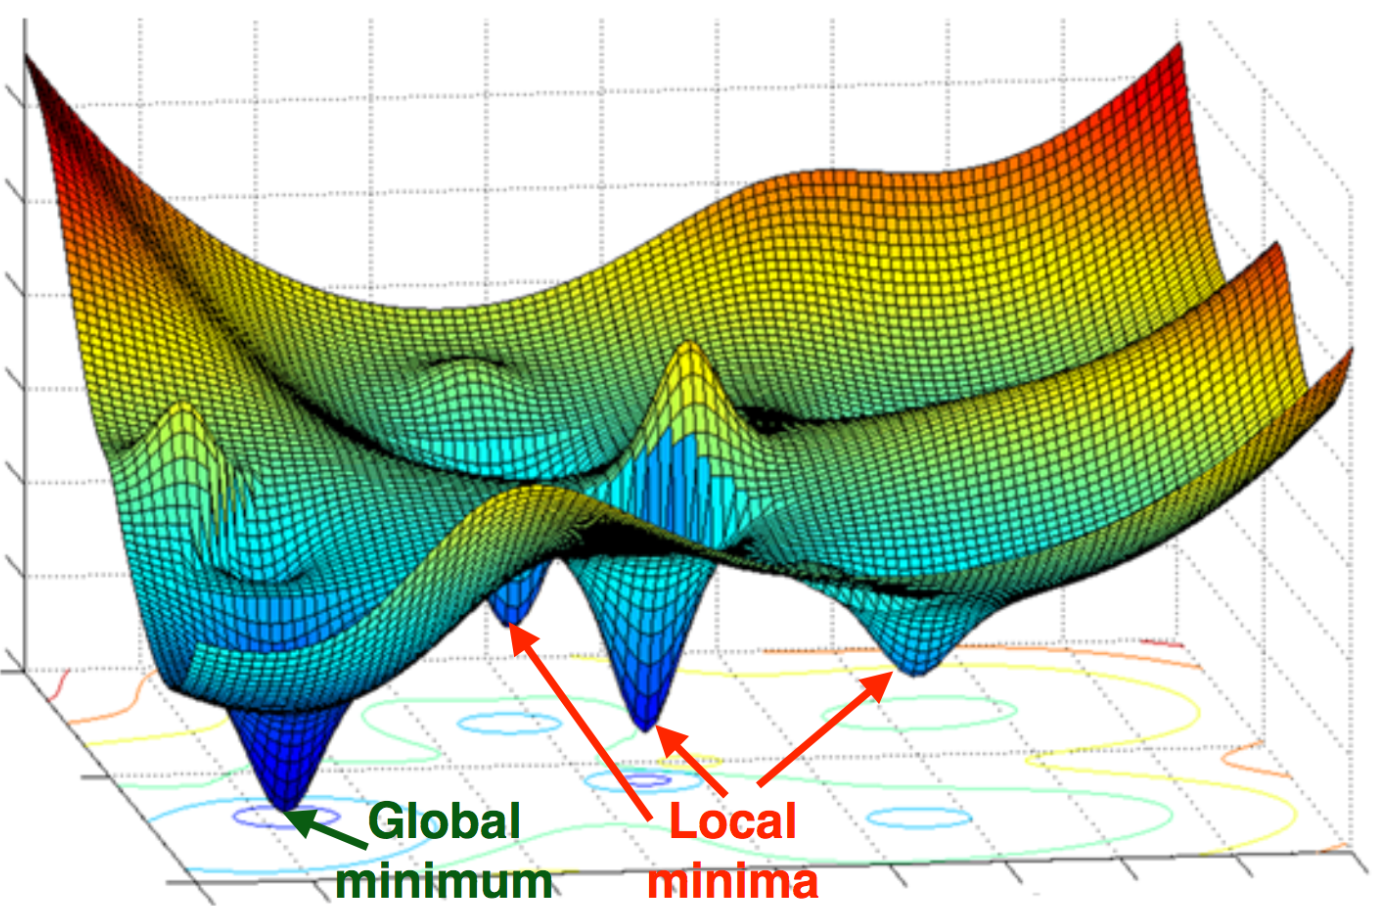
\includegraphics[width=4in]{stuff/minmax.png}
\end{figure}
}

\frame
{
 \frametitle{Sadly, backpropagation (GD) is very weak on Deep NN's}

\begin{itemize}
\item<1-> But if you're gonna, then consider stochastic or mini-batch
\item<2-> You'll be doing many \emph{epochs} (iterations through the data)
\item<3-> And you might wanna explore using \textcolor{blue}{momentum} and \textcolor{red}{velocity} 
\begin{align*}
\textcolor{red}{V^{(t)}} = {}& \textcolor{blue}{\mu} \textcolor{red}{V^{(t-1)}} - \alpha \nabla Cost(W^{(t-1)})\\
W^{(t)} = {}& W^{(t-1)} + \textcolor{red}{V^{(t)}}
\end{align*}
\end{itemize}
\vspace{-1em}
\onslide<3->{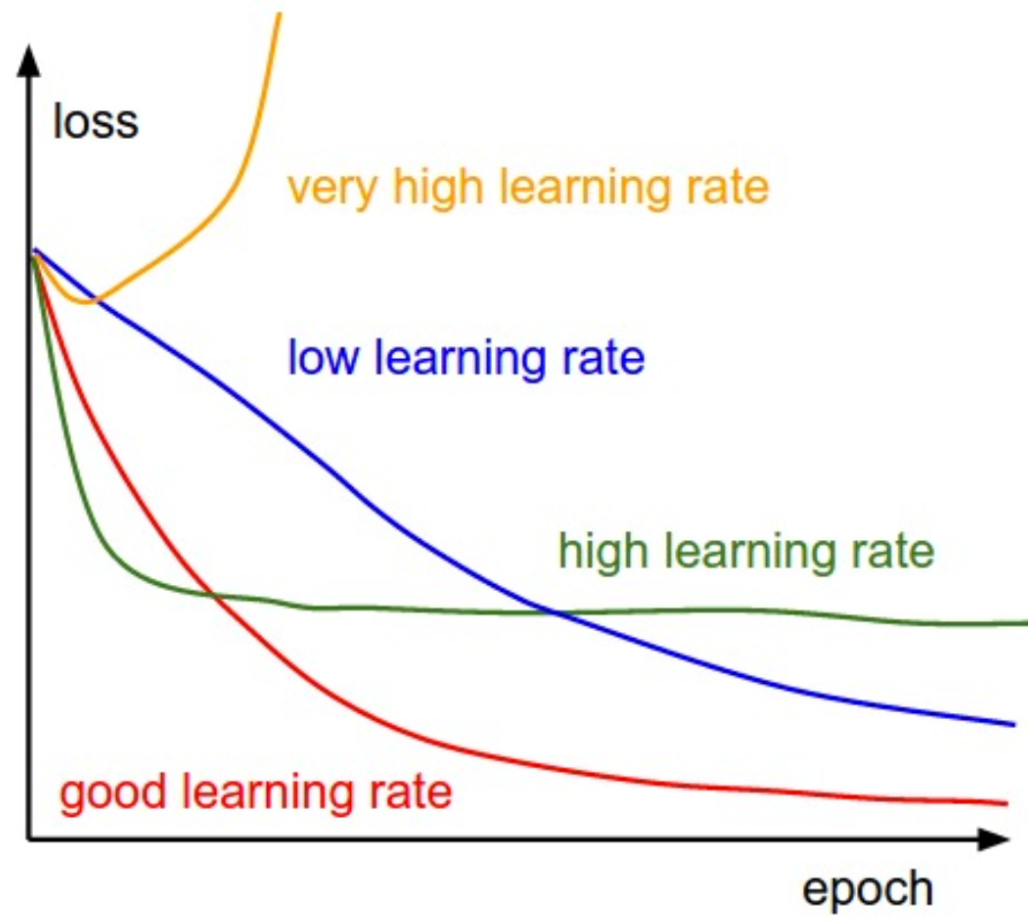
\includegraphics[width=1.8in]{stuff/learnrate.png}$\quad$\raisebox{.9em}{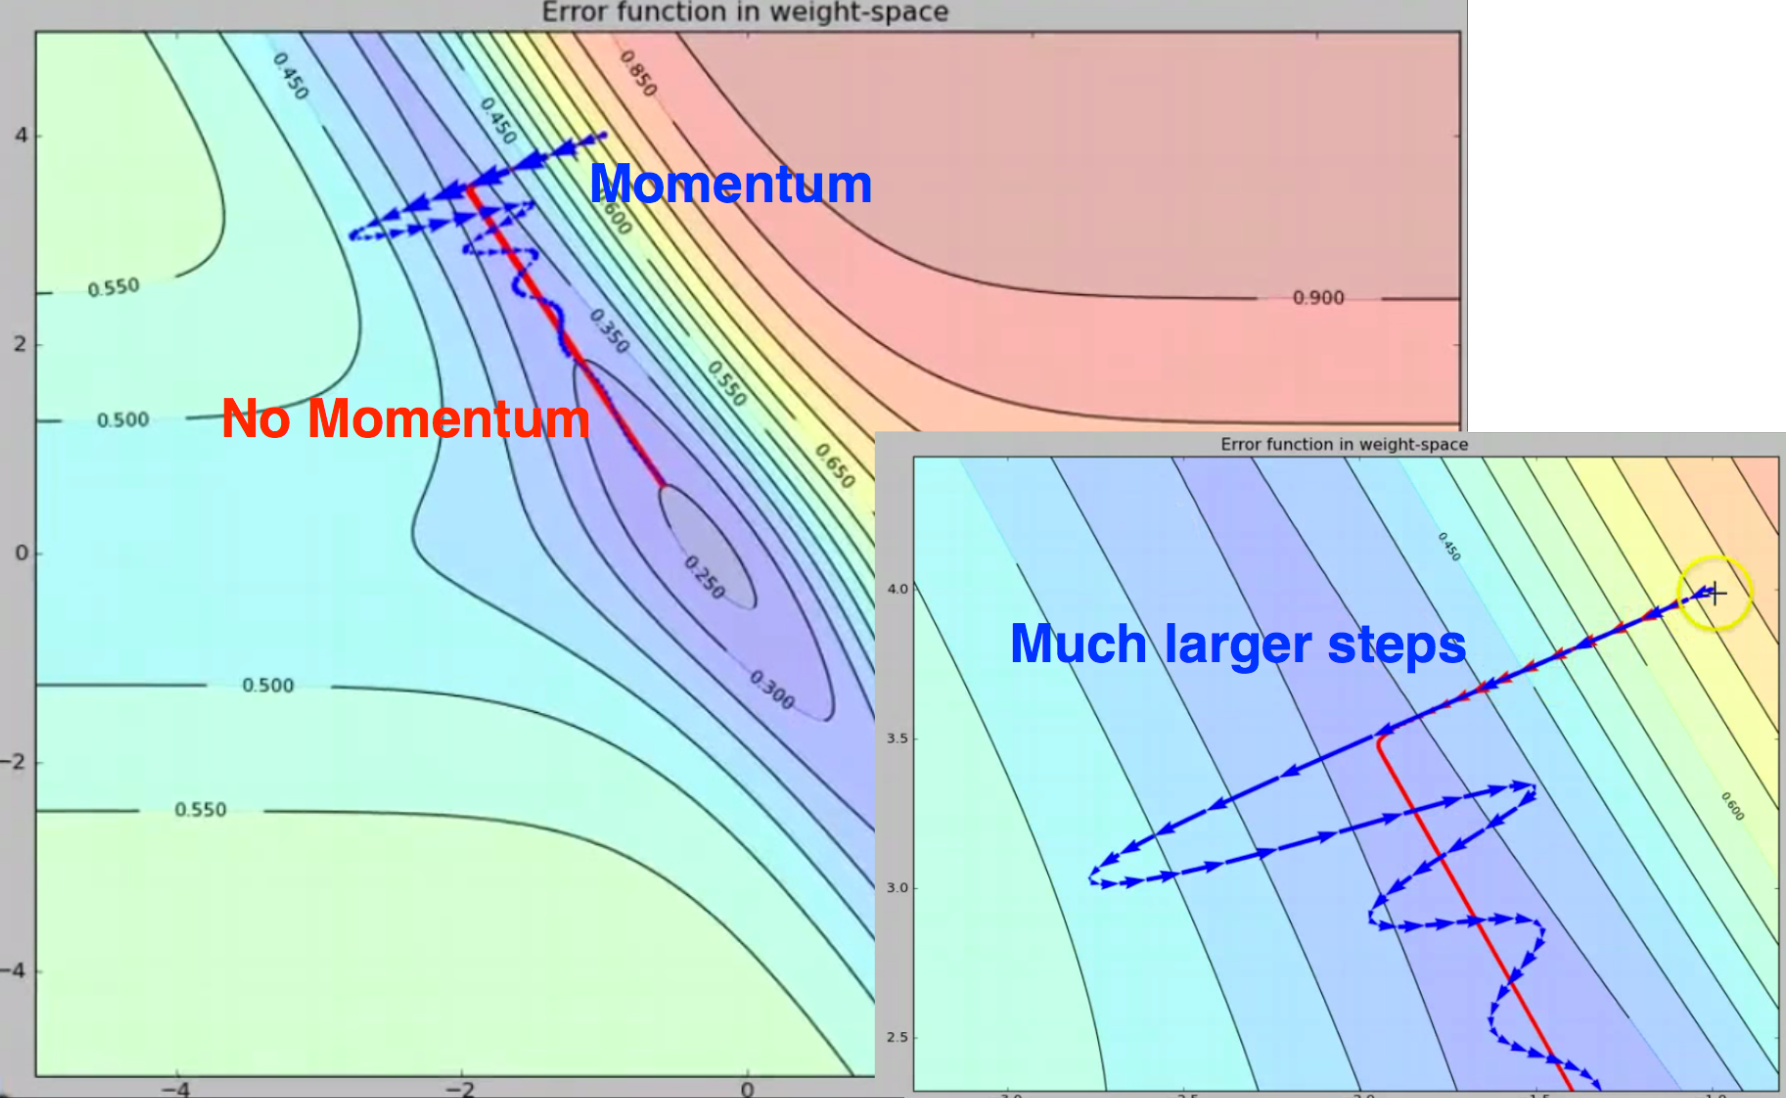
\includegraphics[width=2.4in]{stuff/momentum.png}}}
}

\frame
{
 \frametitle{Sadly, backpropagation (GD) is very weak on Deep NN's}

\begin{itemize} 
\item Not much consensus on designs -- lots of trial and error...
\item<2-> but usually less that 3 hidden layers
\item<3-> fewer outputs than inputs per layer
\item<4-> 2*p neurons (noisy data) to 30*p neurons (perfect signal)
\item<5-> probably rectified linear, perhaps tanh \& \emph{maybe} sigmoid AF's
%\item<6-> and tricks: \\
\end{itemize}
%$\quad$\onslide<6->{\url{research.microsoft.com/pubs/192769/tricks-2012.pdf}}

\onslide<6->{
\begin{figure}
\centering
Here's what you'll actually do:

\LARGE
find an NN paper doing *something like* what you're
trying to do, get theirs to work, and then adapt it to your data
\end{figure}
}

}


\frame
{
 \frametitle{The new type of data}

\begin{figure}
\centering
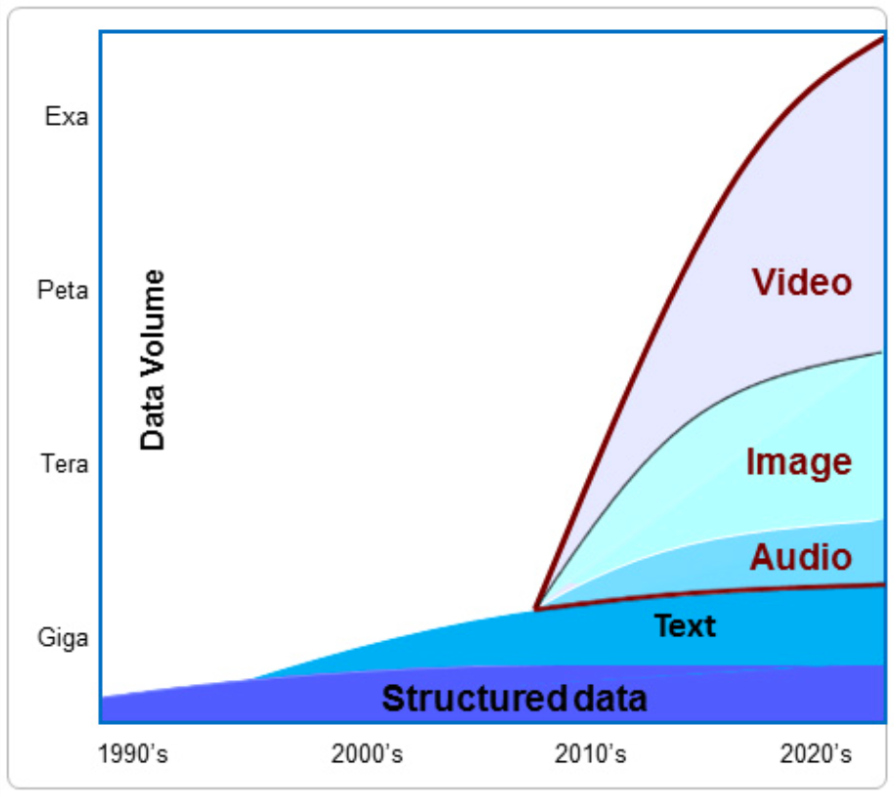
\includegraphics[width=3.5in]{stuff/image_motive.png}
\end{figure}

}


\frame
{
 \frametitle{What data/information is contained in an image?}

\begin{figure}
\centering
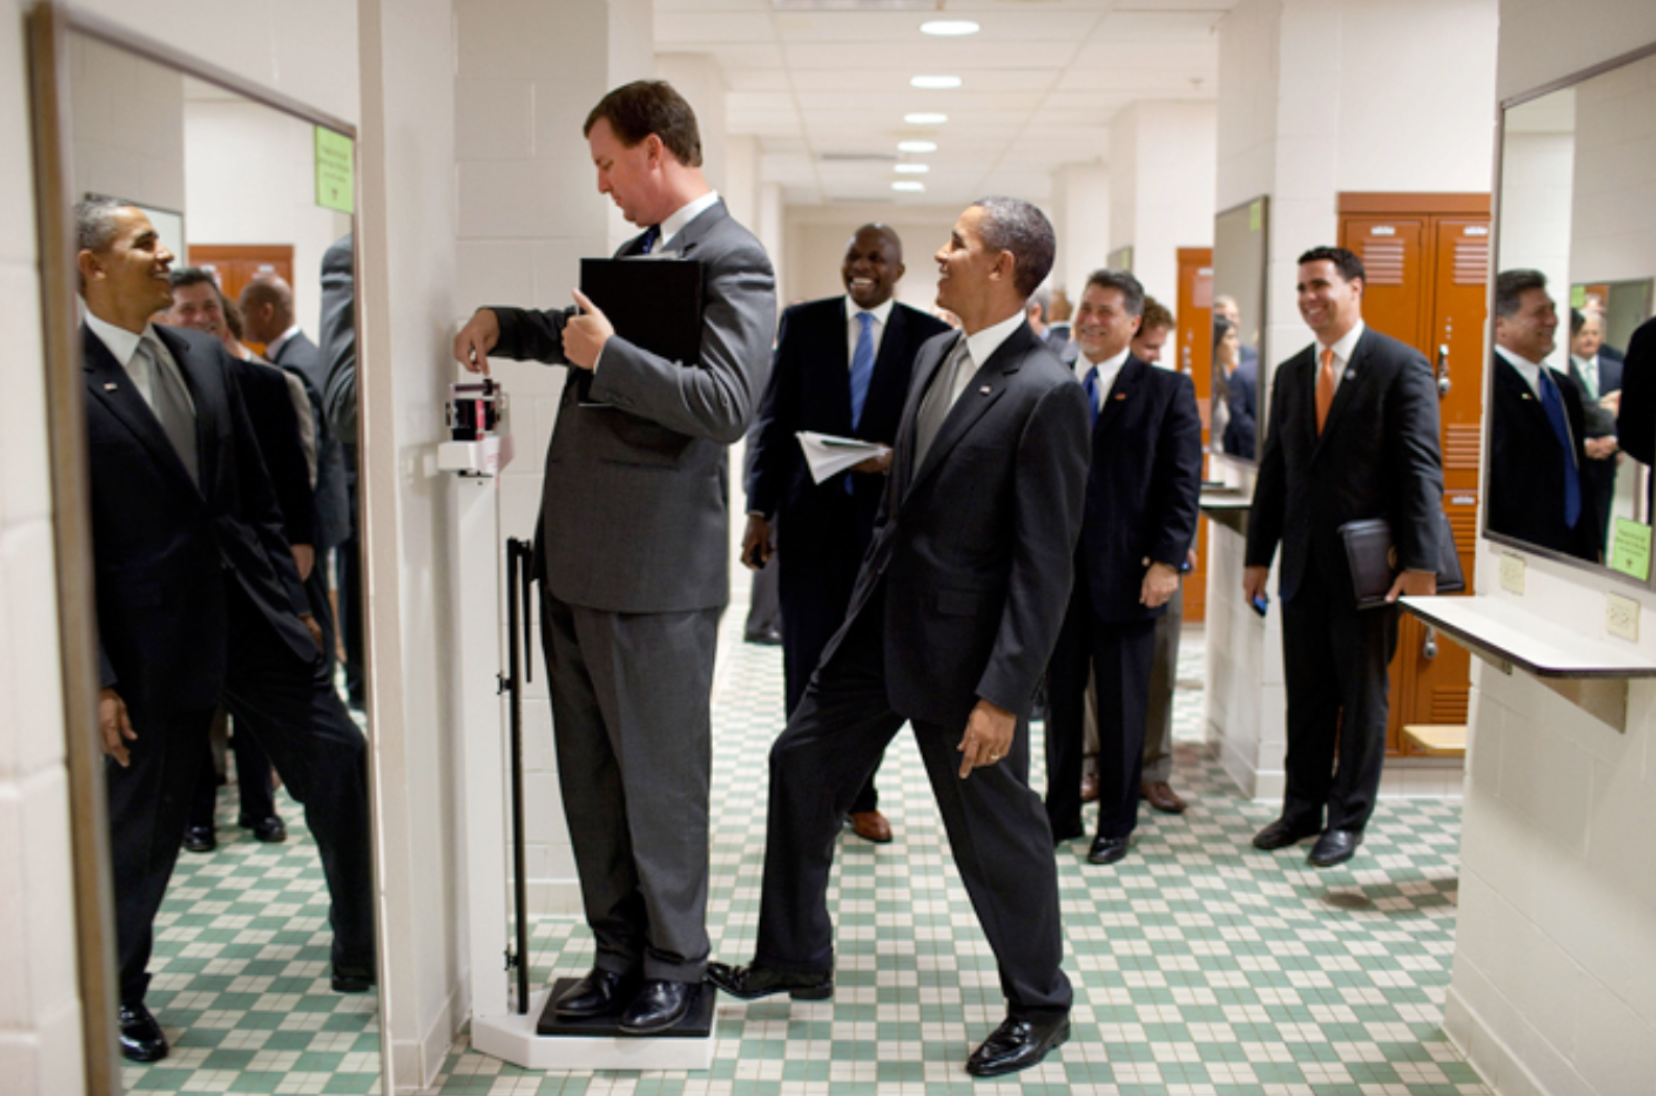
\includegraphics[width=4in]{stuff/obams.png}
\end{figure}

}



\frame
{
\frametitle{What data/information is contained in an image?}

 \newcommand{\rgb}{\textcolor{red}{R}\textcolor{green}{G}\textcolor{blue}{B}}

\Large
A color image is a \emph{tensor}: a matrix of vectors
$$\left[\begin{array}{cccc} \rgb &\rgb &\cdots & \rgb\\ \rgb &\rgb &\cdots & \rgb\\ \vdots & \vdots & \ddots &\vdots \\ \rgb &\rgb &\cdots & \rgb\\\end{array}\right]$$
\normalsize
\hspace{2in} image.shape = (width, height,3)\\${}$\\



\vspace{-.5em}
\onslide<3->{Grayscale (luminescence): $0.2125\textcolor{red}{R} + 0.7154  \textcolor{green}{G} + 0.0721 \textcolor{blue}{B}$}

\onslide<2-3>{\onslide<2>{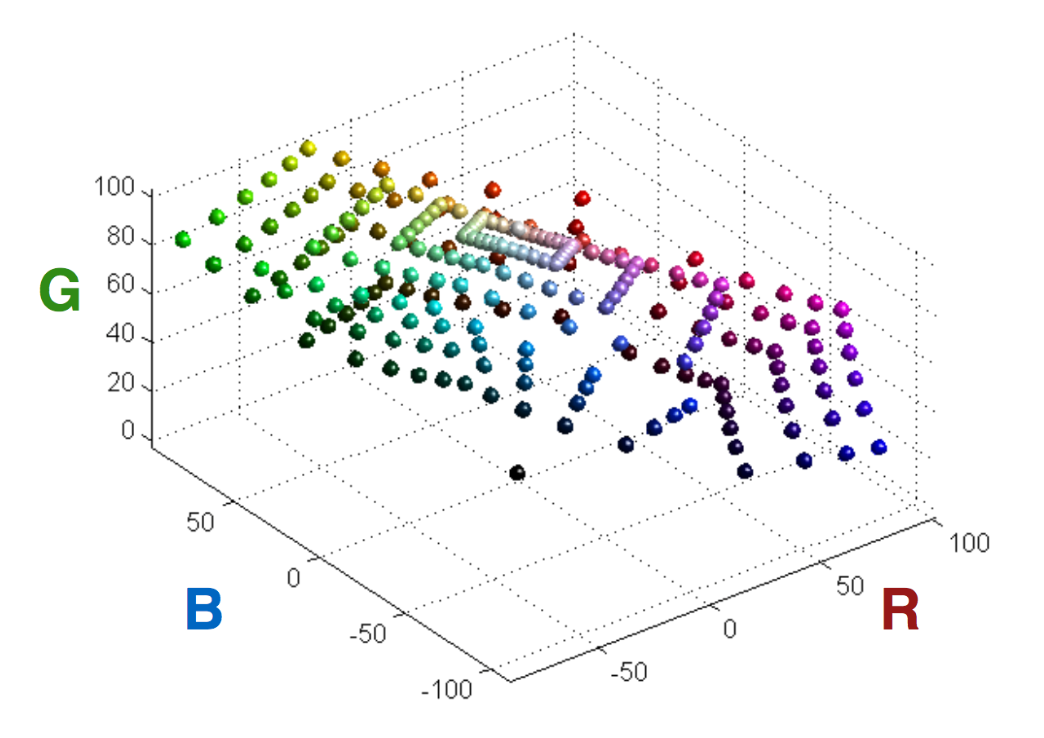
\includegraphics[height=1.5in]{stuff/rgeebee.png}}\only<2>{\raisebox{1em}{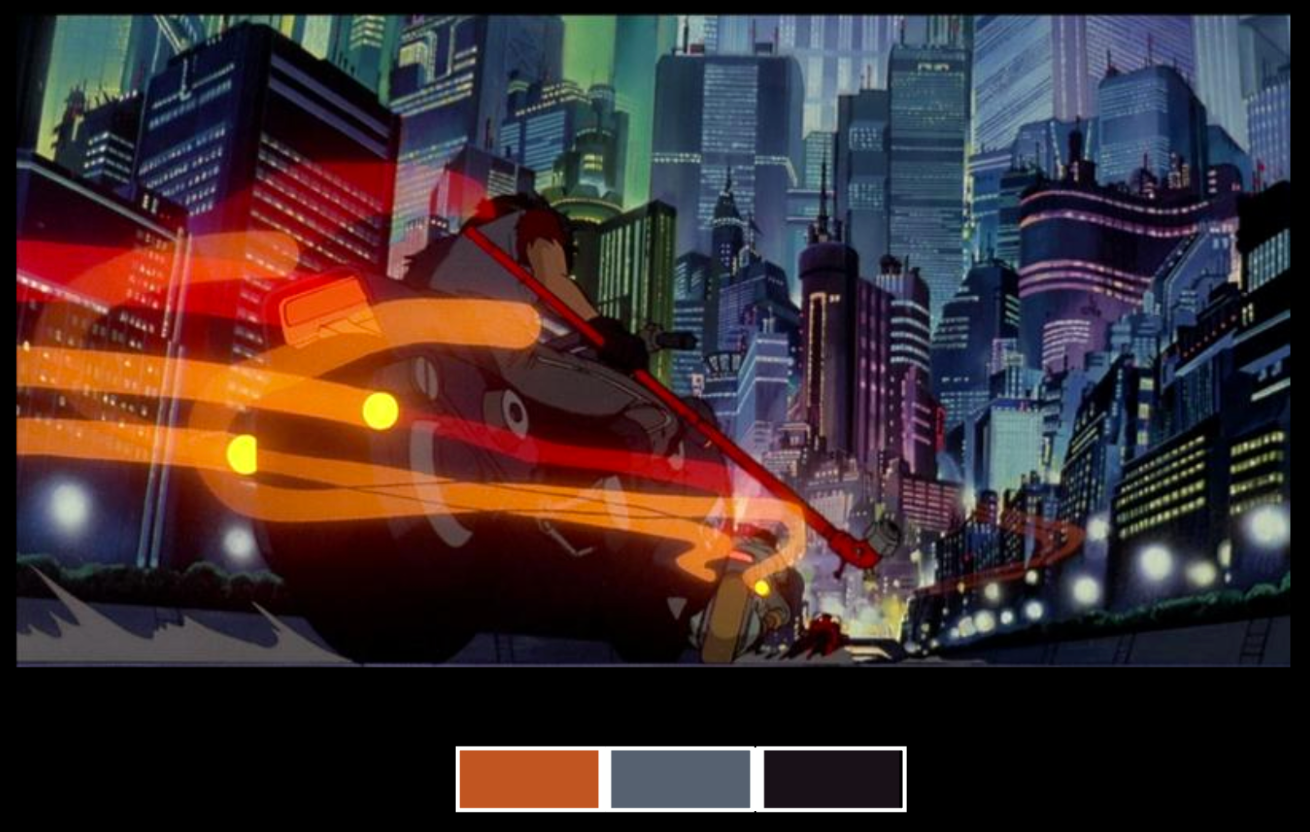
\includegraphics[height=1.2in]{stuff/cool.png}}}\only<3>{\raisebox{1em}{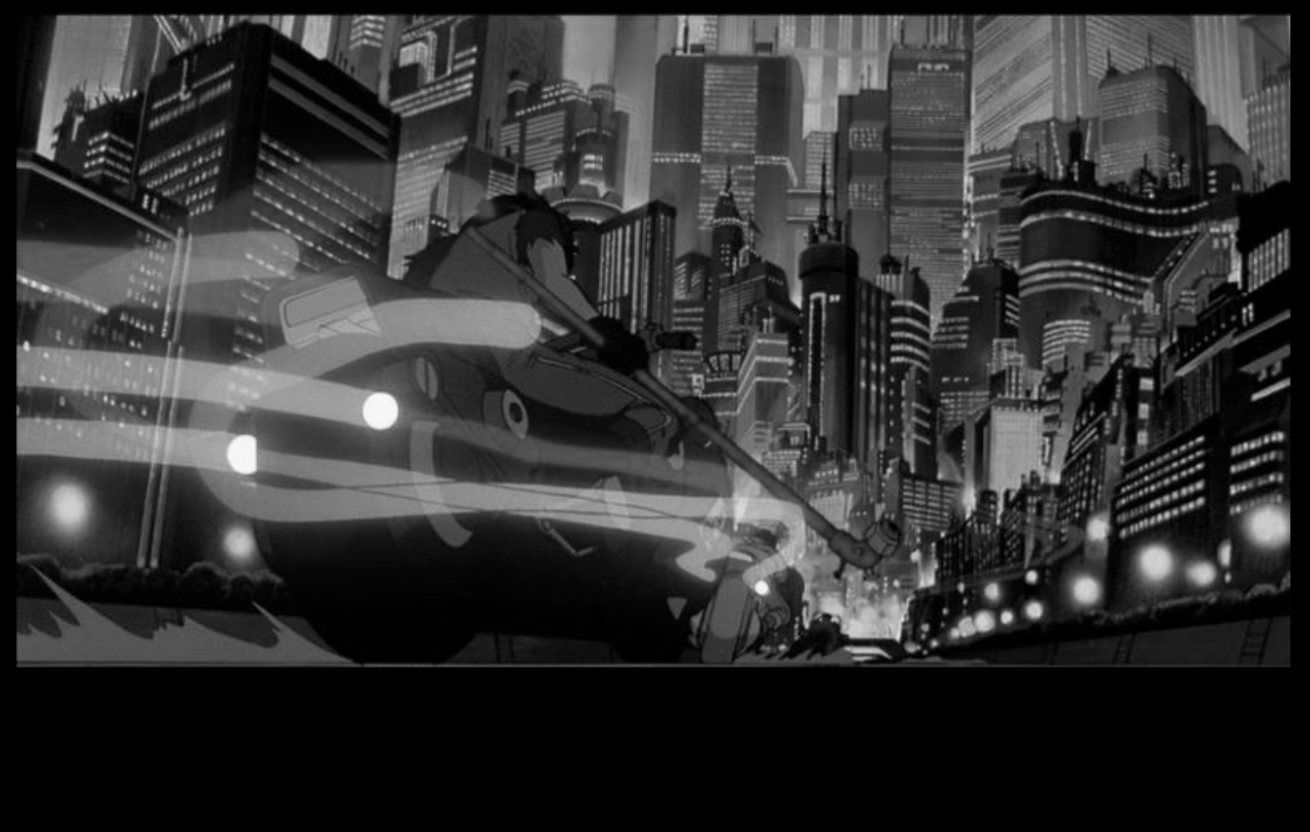
\includegraphics[height=1.2in]{stuff/cool2.png}}}}

\begin{figure}
\centering
\vspace{-1.475in}


\vspace{.02in}

\only<4->{\fbox{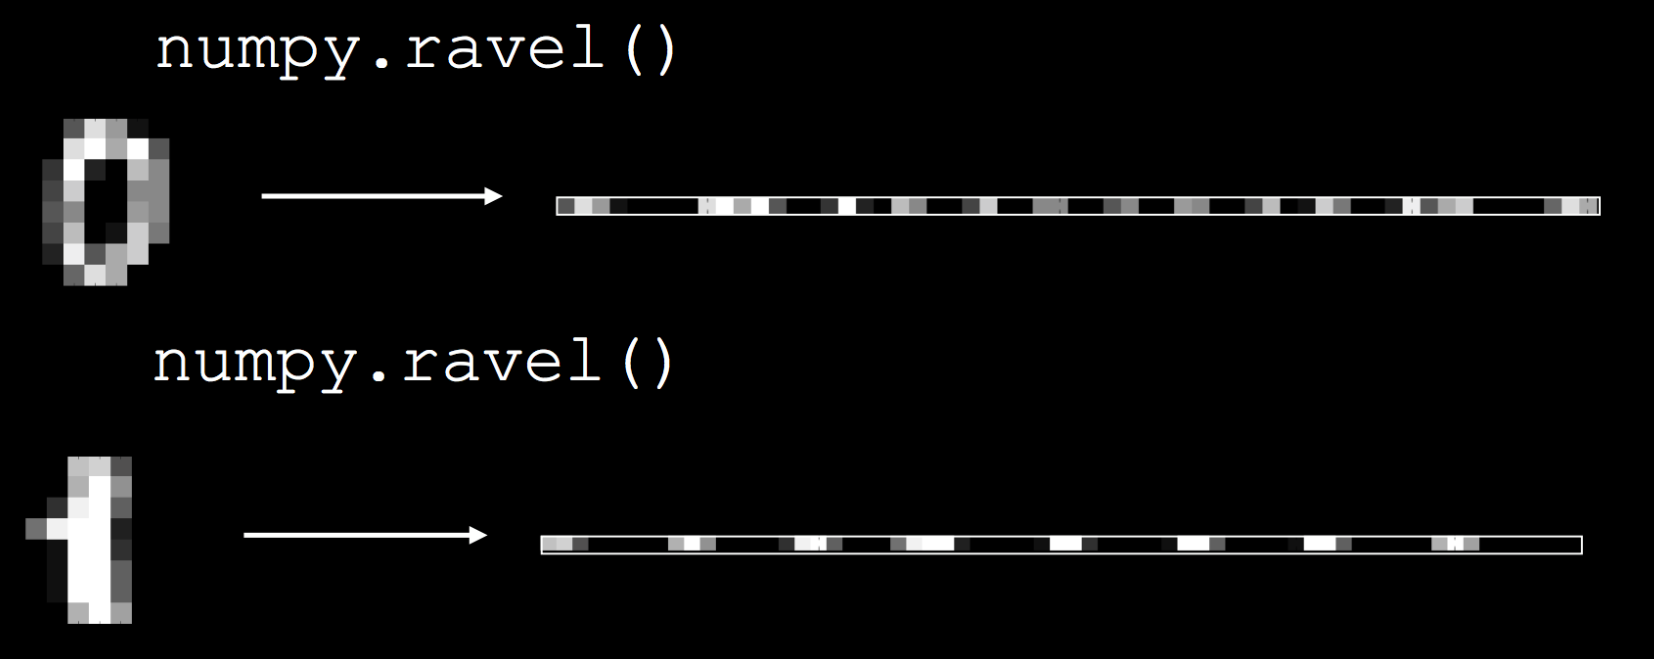
\includegraphics[width=2.15in]{stuff/vectorize.png}}}
\end{figure}
\only<4->{\hspace{1.5in} featurized.shape = (width$\cdot$height$\cdot$3,1)}
\vspace{2in}

}




\frame
{
\frametitle{What data/information is contained in an image?}

$$\hspace{2cm}\begin{array}{c}\textcolor{gray}{\text{image 1}}\\\textcolor{gray}{\text{image 2}}\\\vdots\\\textcolor{gray}{\text{image n}}\\\end{array} \left[\begin{array}{cccc} x_{11} & x_{12} &\cdots & x_{1p}\\ x_{21} & x_{22} &\cdots & x_{2p}\\ \vdots & \vdots & \ddots &\vdots \\ x_{n1} & x_{n2} &\cdots & x_{np}\\\end{array}\right]
\overset{\text{Predict}}{\Longrightarrow} \overset{\text{Image Label}}{\left[\begin{array}{c}Y_1\\Y_2\\\vdots\\Y_n\\\end{array} \right]}
$$



\begin{columns}
\begin{column}{.15\textwidth}
%\vspace{1.25em}
\onslide<3->{
\includegraphics[width=1.1in]{stuff/down.png}}\\

\onslide<3->{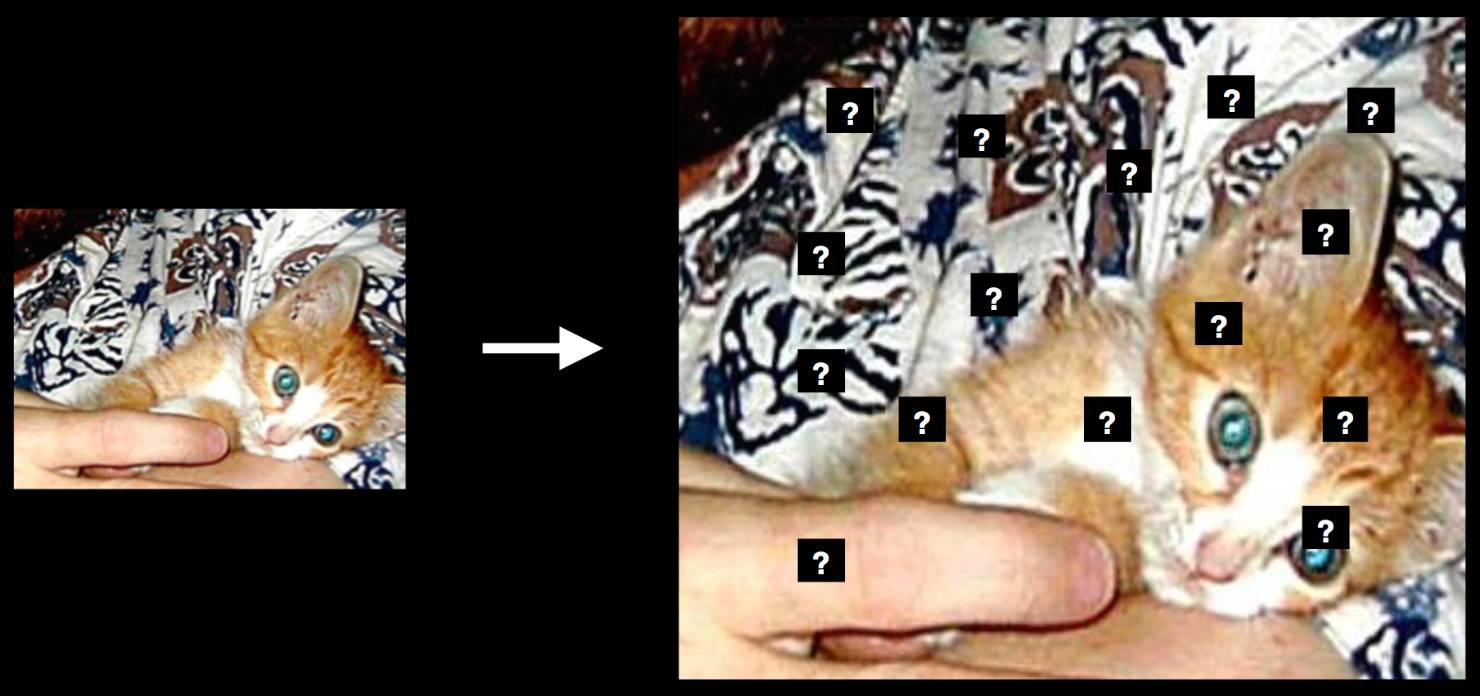
\includegraphics[width=1.1in]{stuff/up.png}} \\

\onslide<3->{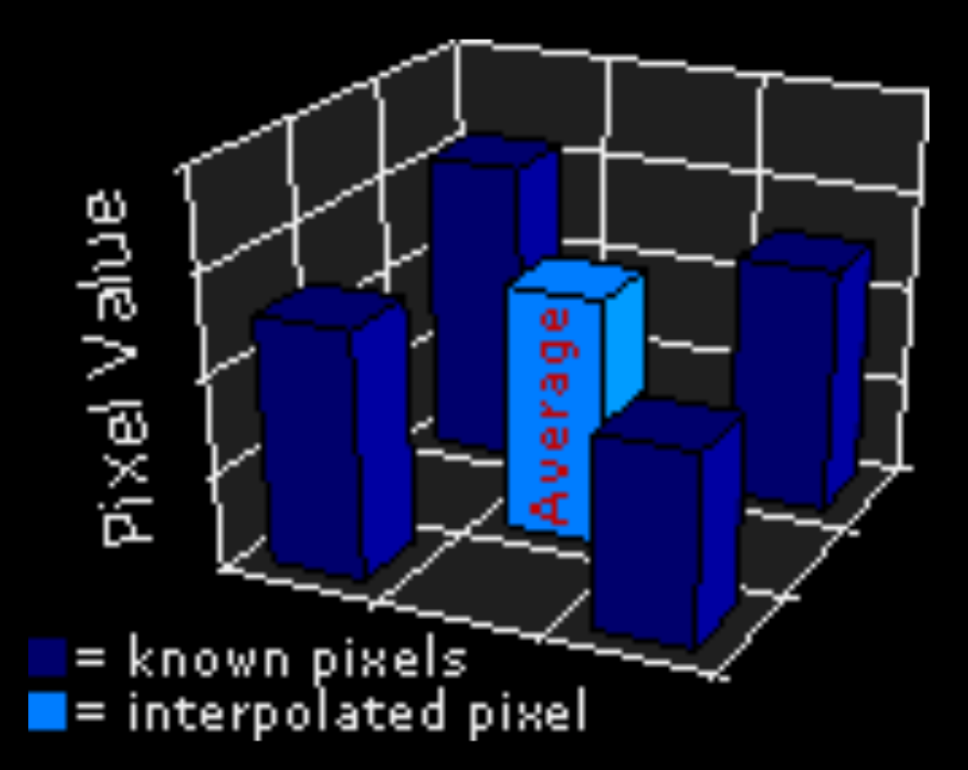
\includegraphics[width=1.1in]{stuff/interp.png}}

\end{column}
\begin{column}{.55\textwidth}
\onslide<2->{{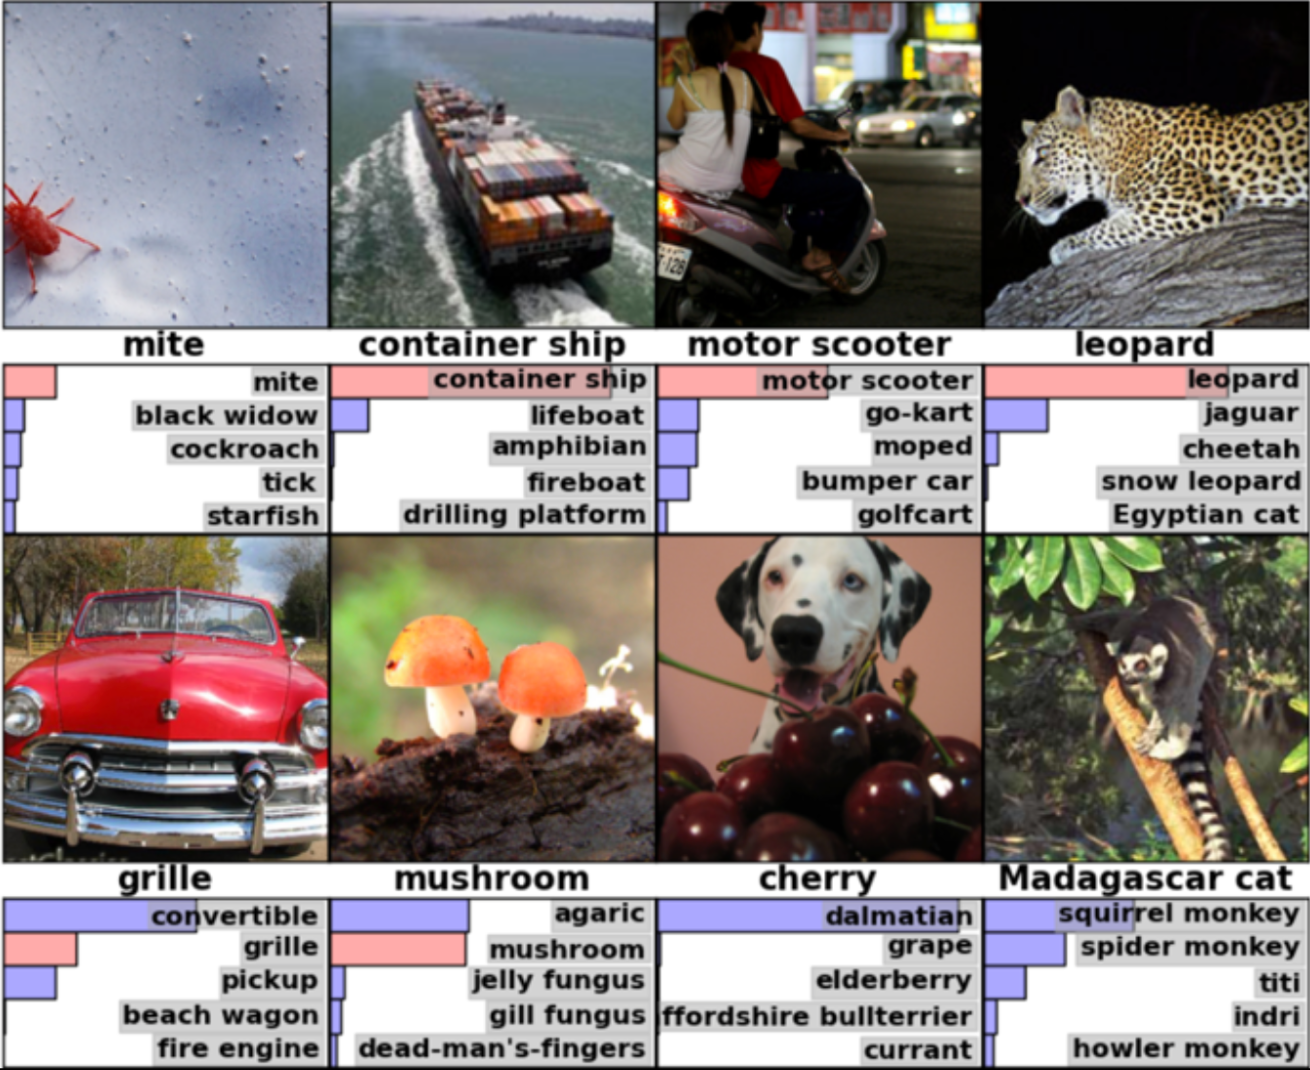
\includegraphics[width=2.45in]{stuff/pattern_rec.png}}}

\end{column}
\end{columns}

}


\frame
{
%MNIST
 \frametitle{NNs are the best at identifying patterns in complex data}

\begin{figure}
\centering
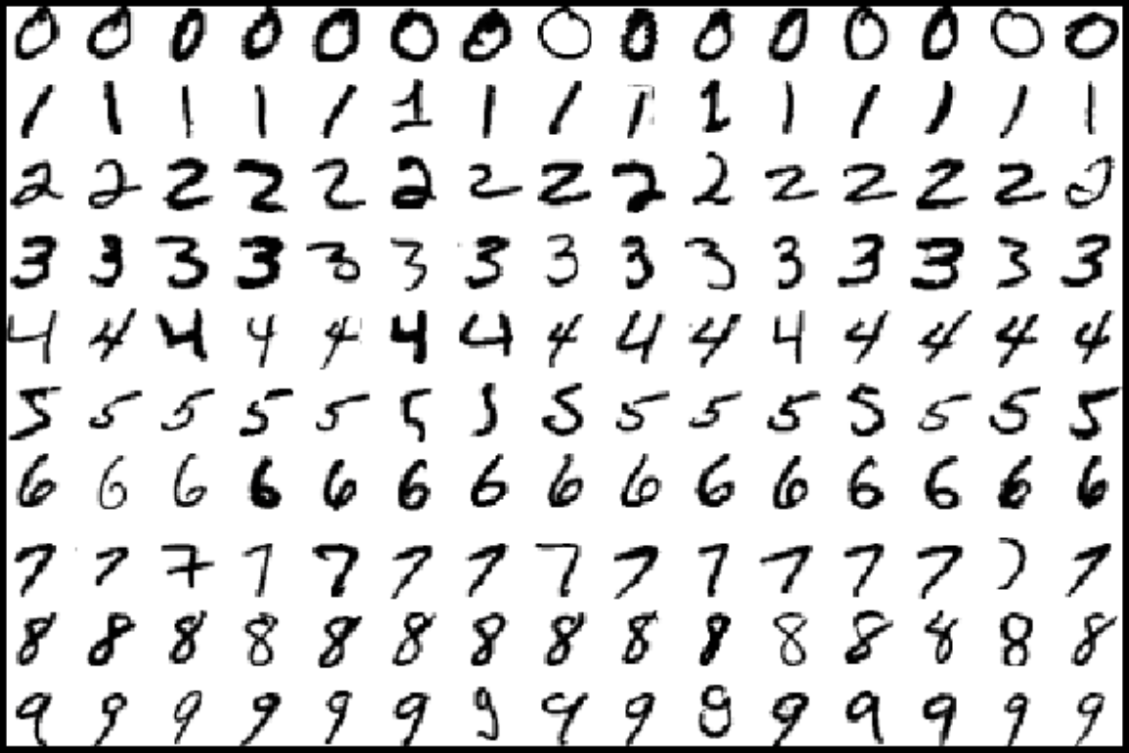
\includegraphics[width=2.25in]{stuff/nums.png}

\begin{tabular}{lr}
\\
Classifier & Test Error Rate \\
Large and Deep Convolutional Network & 0.33\%\\
SVM with degree 9 polynomial kernal & 0.66\% \\
Gradient boosted stumps on Haar features & 0.87\%
\end{tabular}
\end{figure}

Neural networks can recognize patterns from complex, heavy-tailed inputs such as image, audio, video, text, and human speech data 
}



\frame
{
 \frametitle{Image Processing}
 
\begin{itemize}
\item Remove unnecessary details to allow for better\\
generalization of images to image classes\\
\end{itemize}

$$ x_i \rightarrow y_i : \underset{\boldsymbol y}{\text{argmin}} \quad \underset{Fidelity}{\frac{1}{2}\sum(x_i -y_i)^2} + \lambda \underset{Variation}{\sum |y_{i+1}-y_i|}$$

\begin{figure}
\centering
{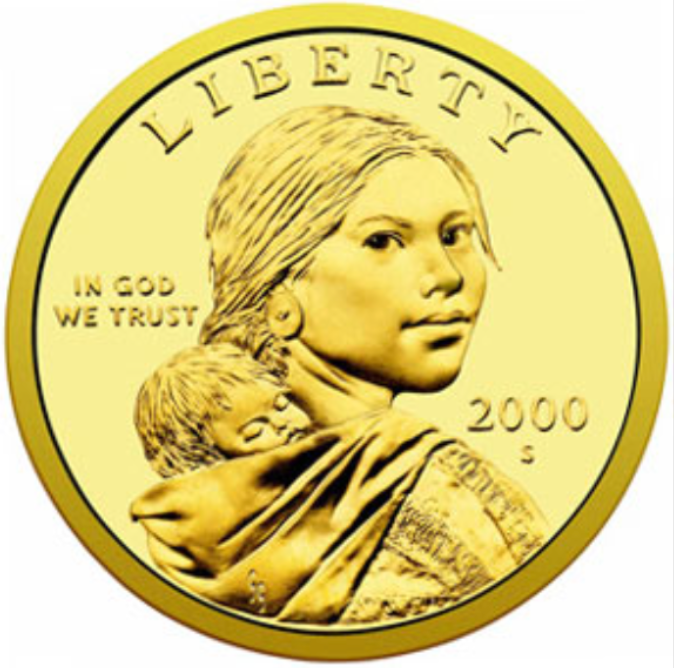
\includegraphics[width=1.75in]{stuff/dn1.png}}$\;\;${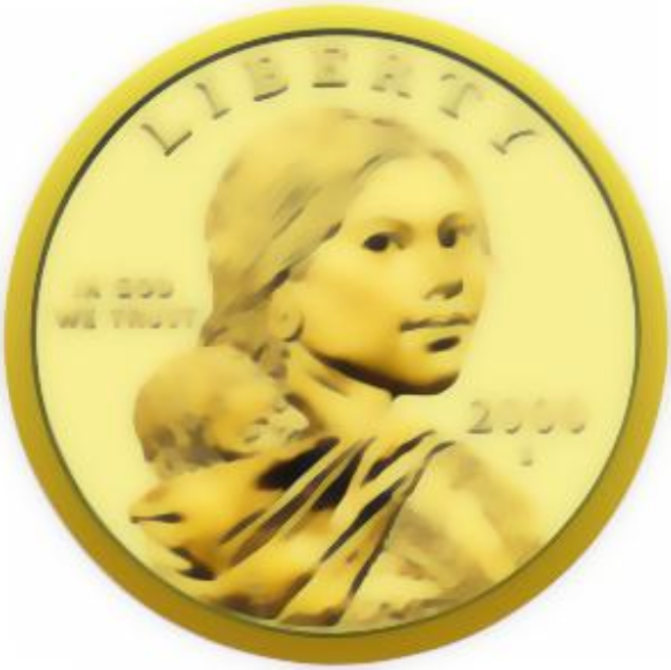
\includegraphics[width=1.75in]{stuff/dn2.png}}
\end{figure}

}



\frame
{
 \frametitle{Convolutional Kernel}
 
\begin{itemize}
\item<1-> Spatial proximity \emph{and pixel agreement (bi-lateral)}

\begin{figure}
\centering
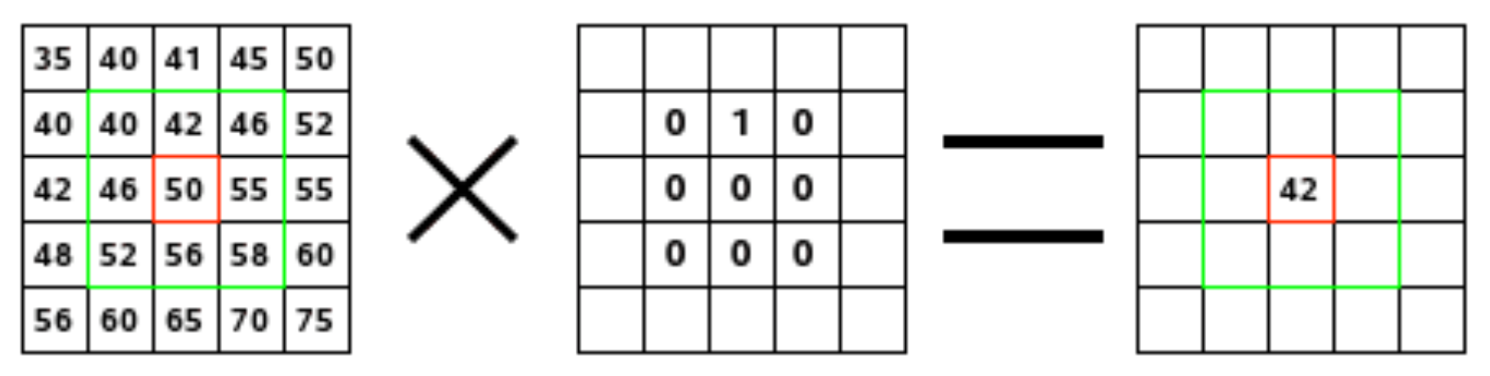
\includegraphics[height=.75in]{stuff/convolution.png}\\${}$\\${}$\\
\vspace{-.075in}
\vspace{-1.025in}
\onslide<2->{\hspace{2.83cm}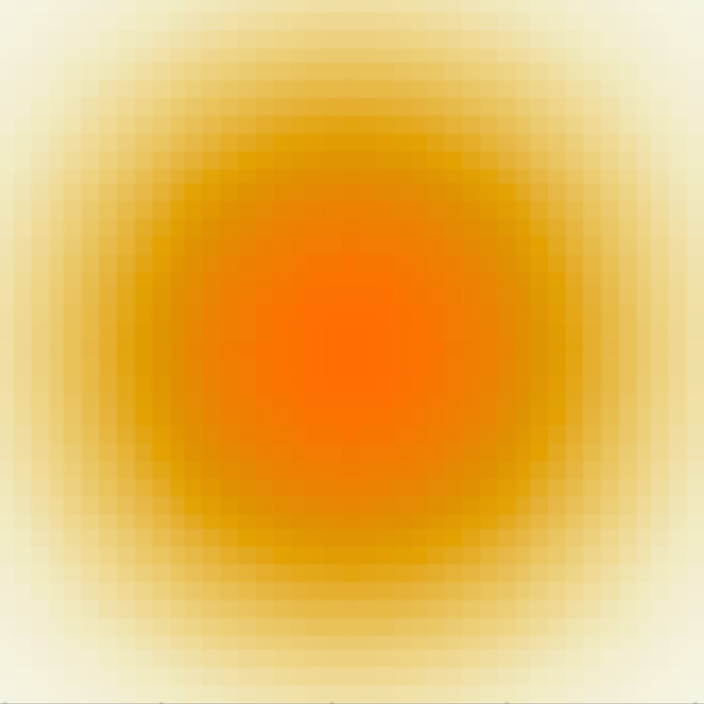
\includegraphics[height=.675in]{stuff/gaussian_convo.png}\textcolor{white}{..-....-..}
\includegraphics[height=.675in]{stuff/gradientZ.png}}

%\vspace{-.95in}
%\onslide<3>{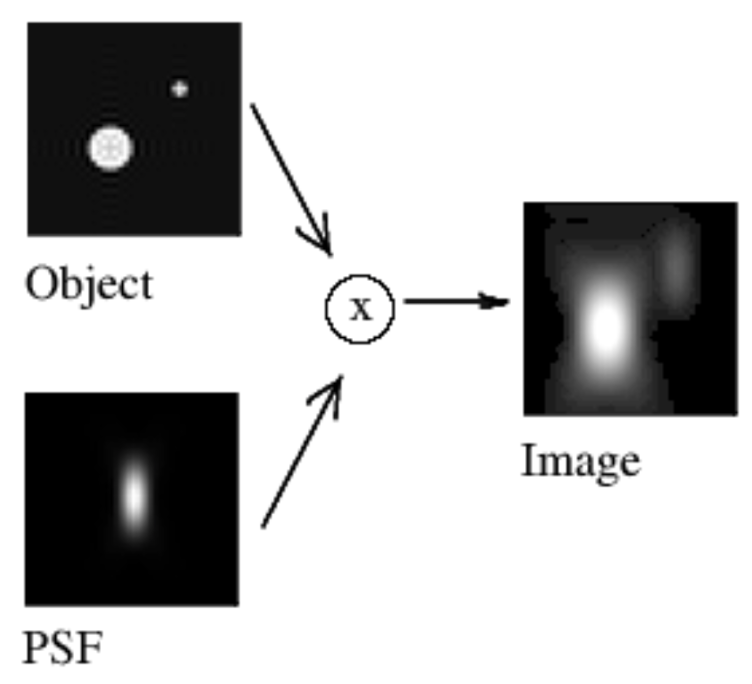
\includegraphics[height=2.1in]{convo2.png}\textcolor{white}{..-..-..-..-.--..}}


\vspace{.25in}
\onslide<3->{\fbox{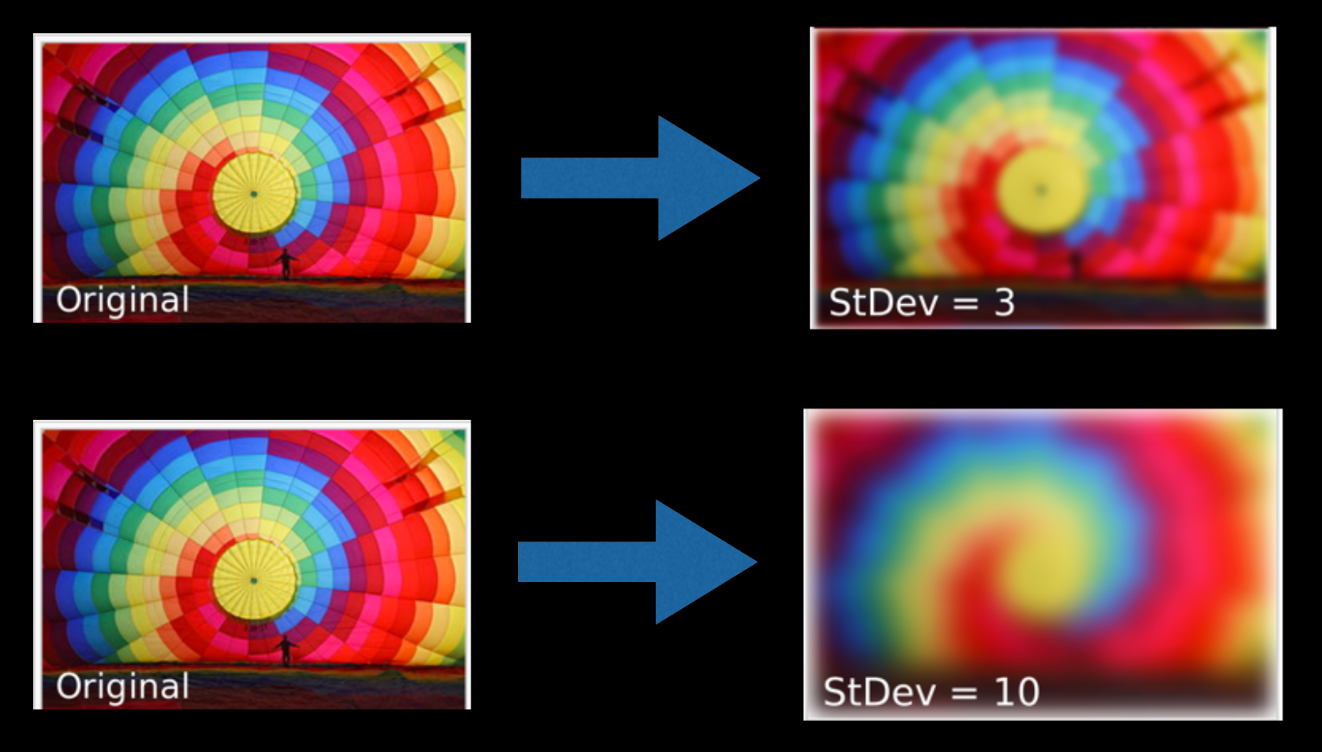
\includegraphics[width=2.9in]{stuff/smosh.png}}}

\end{figure}
\end{itemize}
}




\frame
{
 \frametitle{Convolutional Kernel}

It may be easier to identify objects if we just consider the edges


\begin{figure}
\centering
\fbox{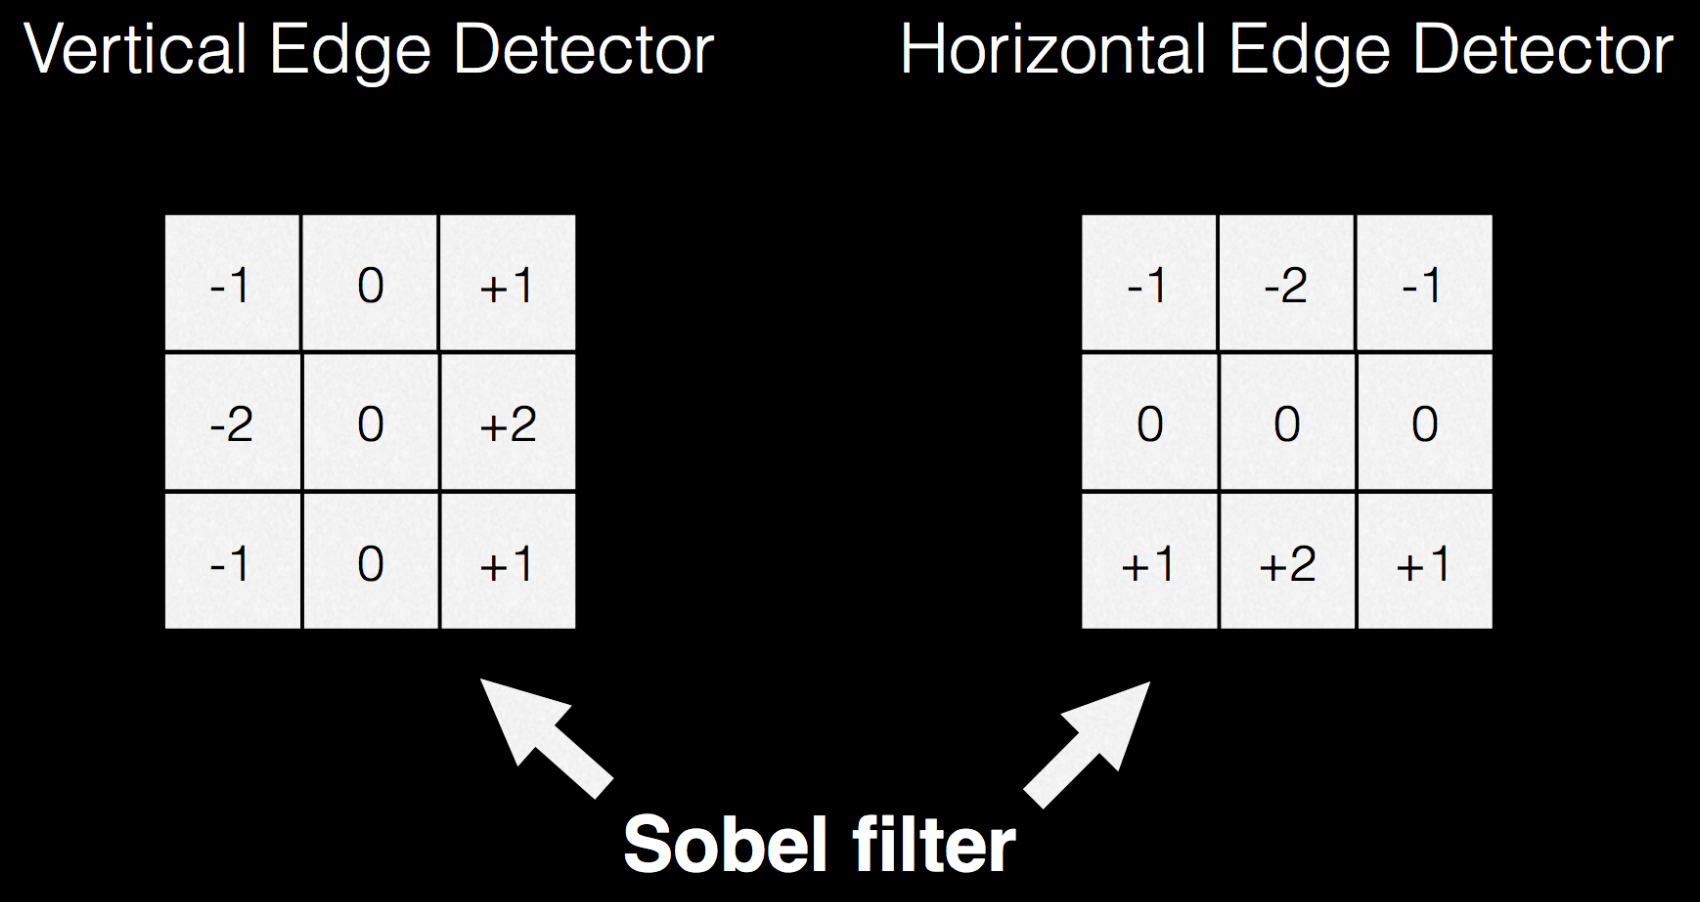
\includegraphics[height=1.12in]{stuff/convol2.png}} \fbox{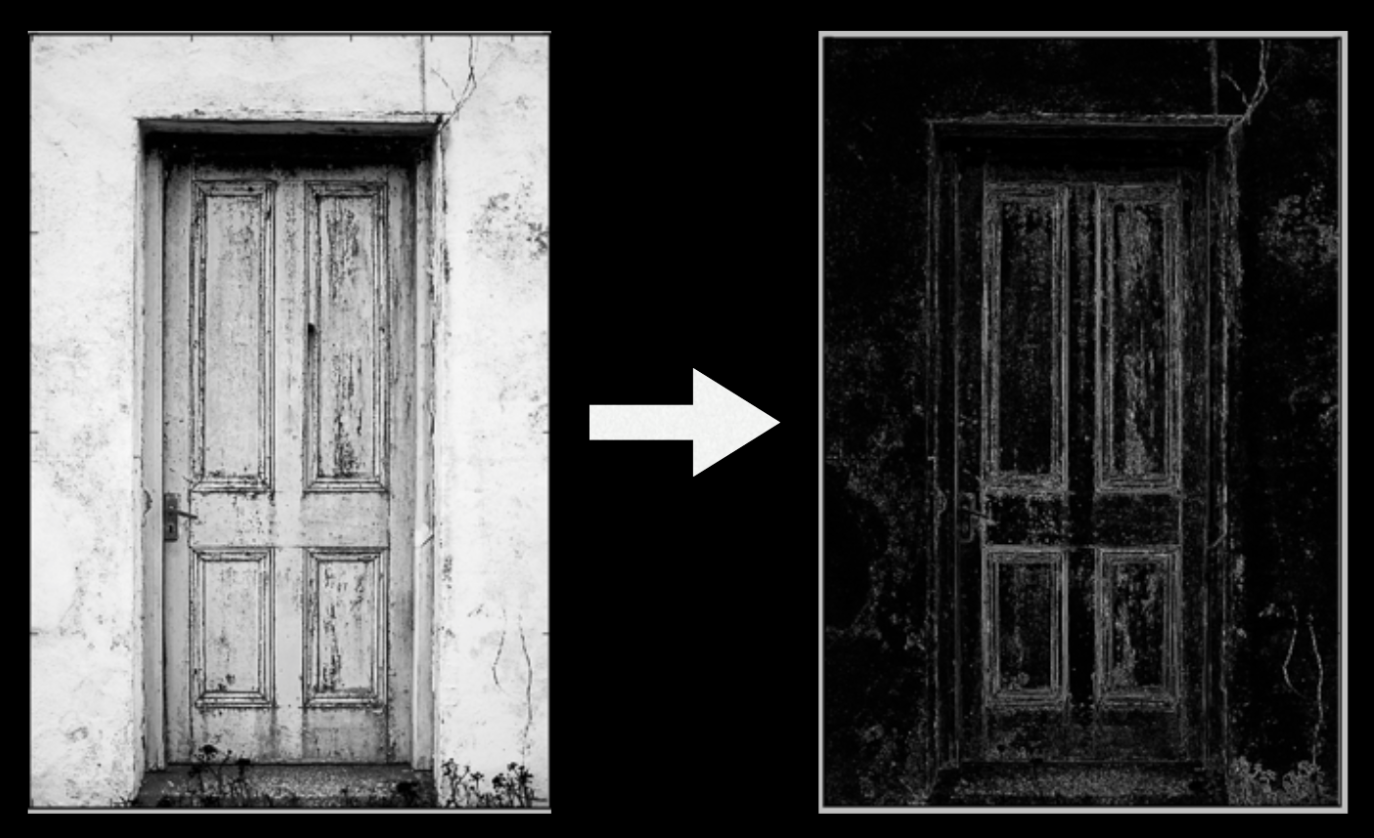
\includegraphics[height=1.12in]{stuff/convol3.png}}
\end{figure}

\vspace{-.05in}
\onslide<2->{
\begin{figure}
\centering
{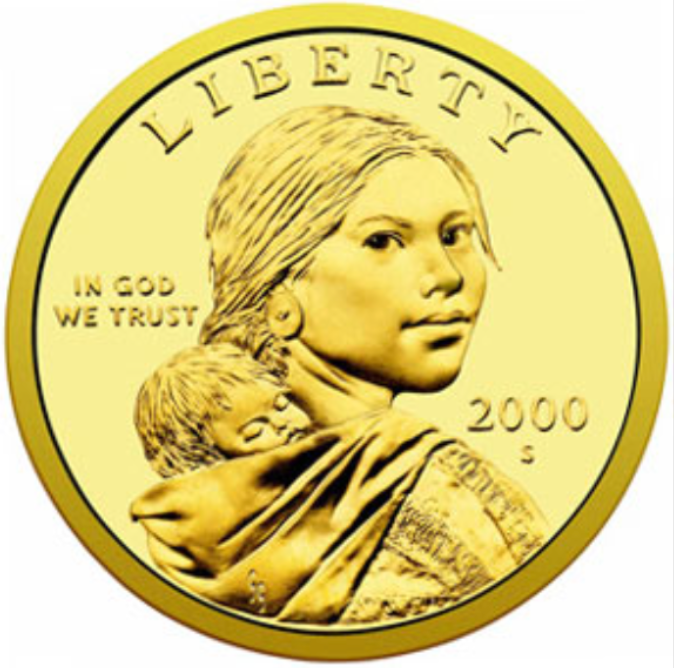
\includegraphics[width=1.25in]{stuff/dn1.png}}$\;${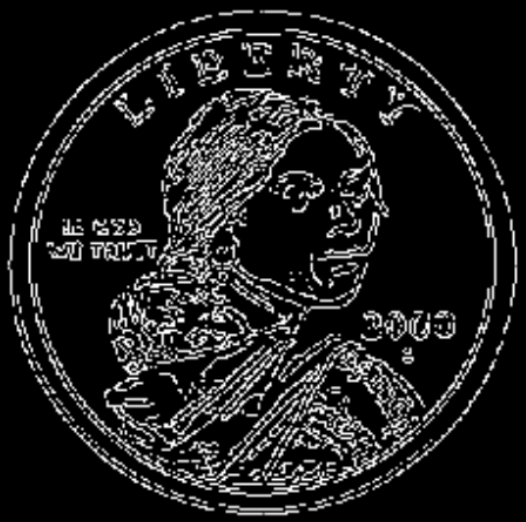
\includegraphics[width=1.25in]{stuff/dn3.png}}$\;${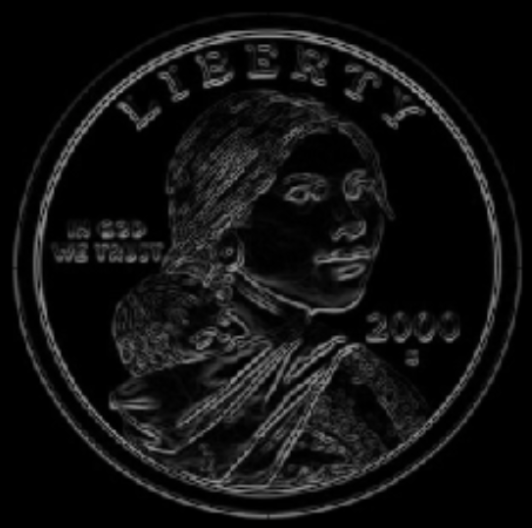
\includegraphics[width=1.25in]{stuff/dn4.png}}
\end{figure}

\vspace{-.2in}
\hspace{11.5em}Canny Filter\hspace{3.5em}Sobel Filter}

}


%We may be able to use intensity gradients for feature ascertainment
%\begin{figure}
%\centering
%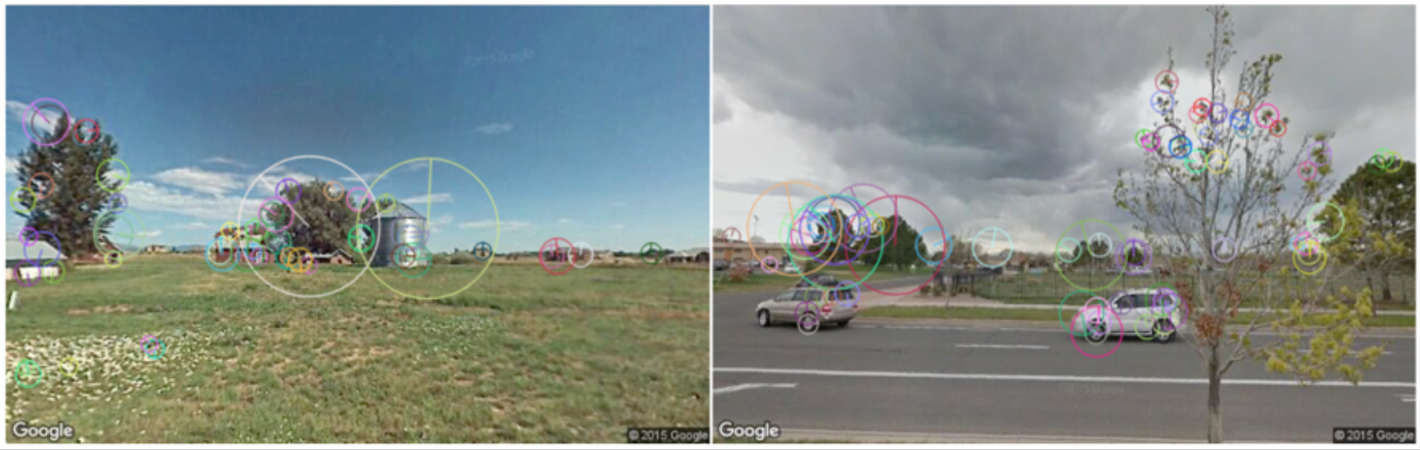
\includegraphics[height=1.3in]{intgrad.png}
%\end{figure}







\frame
{
 \frametitle{Convolutional Kernel}

\begin{columns}
\begin{column}{.25\textwidth}
{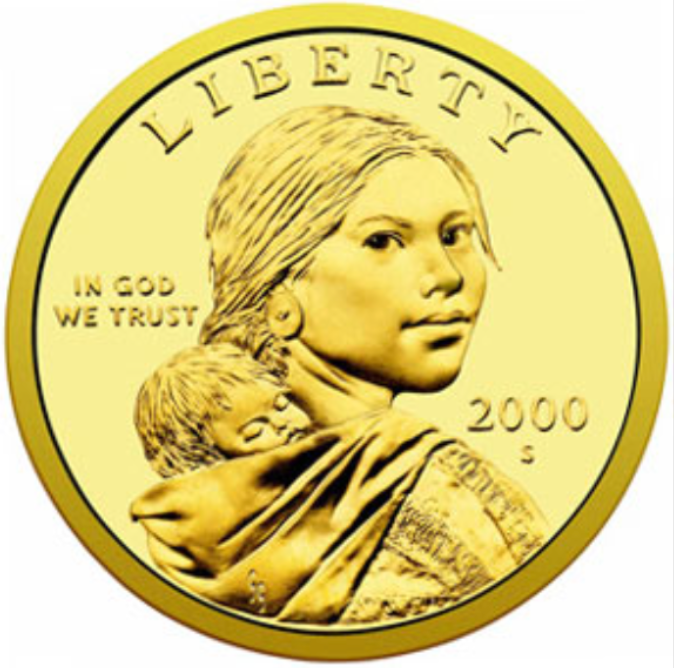
\includegraphics[height=1.2in]{stuff/dn1.png}}\\{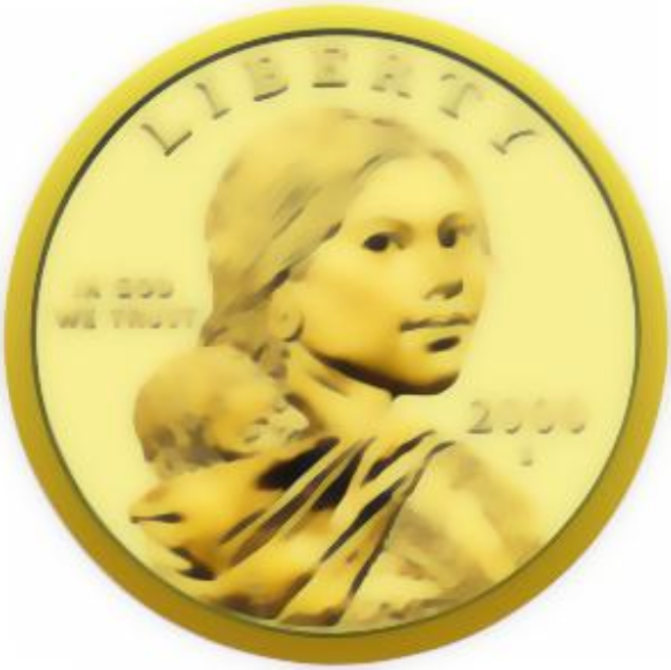
\includegraphics[height=1.2in]{stuff/dn2.png}}\
\end{column}
\begin{column}{.75\textwidth}
\fbox{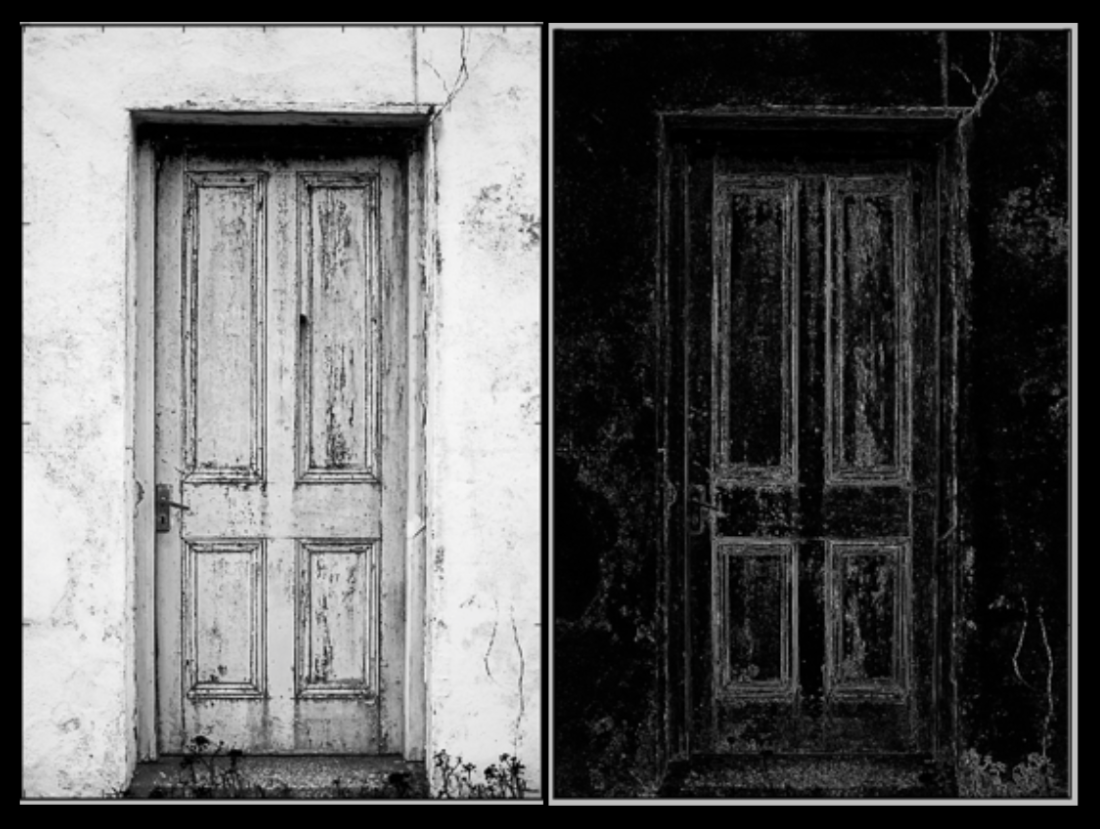
\includegraphics[height=2.25in]{stuff/convol10.png}}
\end{column}
\end{columns}


}



 


\frame
{
 \frametitle{Convolutional Kernel}

Recall that a convolution matrix (or kernel or mask) in image processing is a small matrix 
that can be used to blur, sharpen, emboss, detect edges, etc. through \emph{convolutions}
with an image 


\begin{figure}
\centering
\fbox{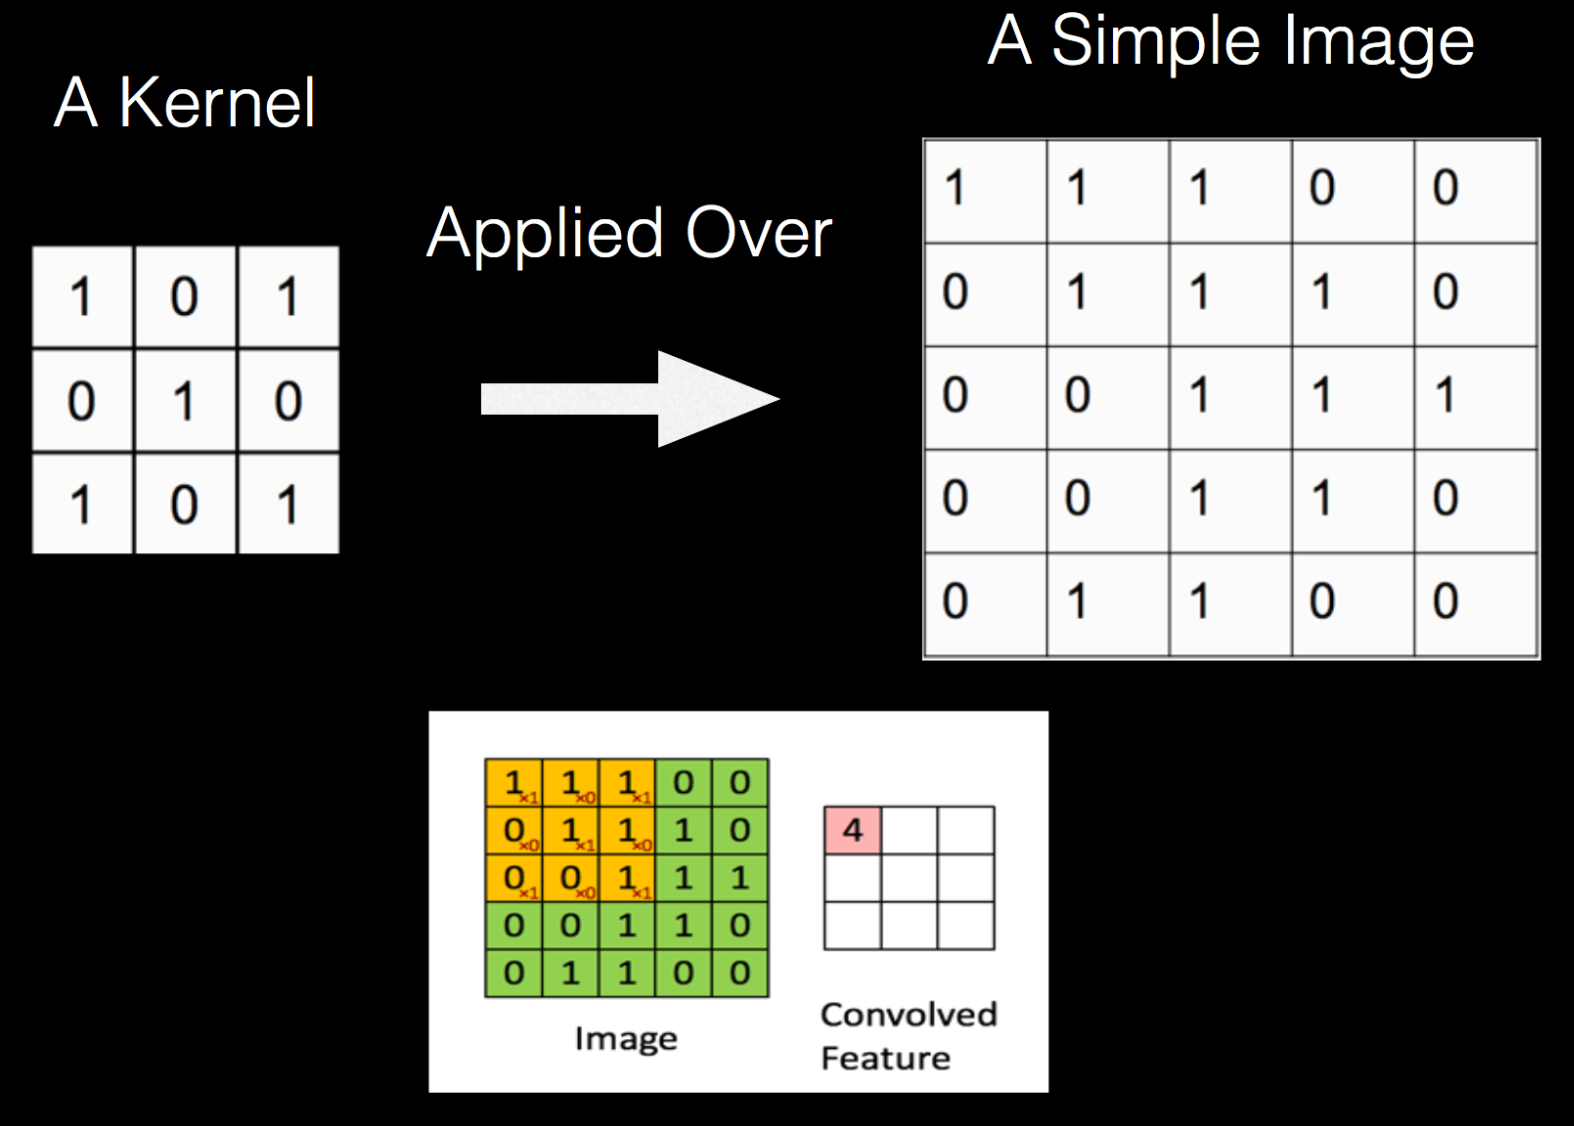
\includegraphics[width=3in]{stuff/convol1.png}}
\end{figure}

}



\frame
{
 \frametitle{idea: \emph{denovo} kernels}

\begin{figure}
\centering
\Huge
Can NN's learn their own convolution matrices? \onslide<2->{\textcolor{red}{Yep.}}

\vspace{.25in}
 \onslide<2->{$\quad$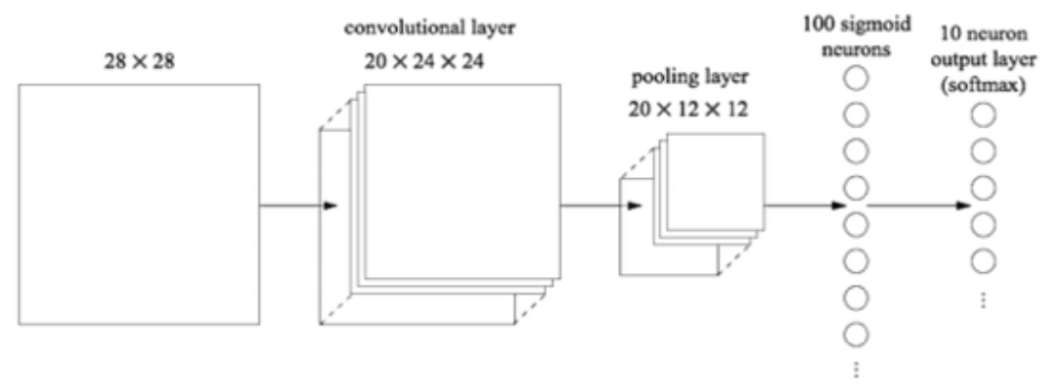
\includegraphics[width=3in]{stuff/convol4.png}}\textcolor{white}{hh}

\end{figure}

}

\frame
{
 \frametitle{Convolutional Neural Network (CNN)}

\begin{figure}
\centering
\fbox{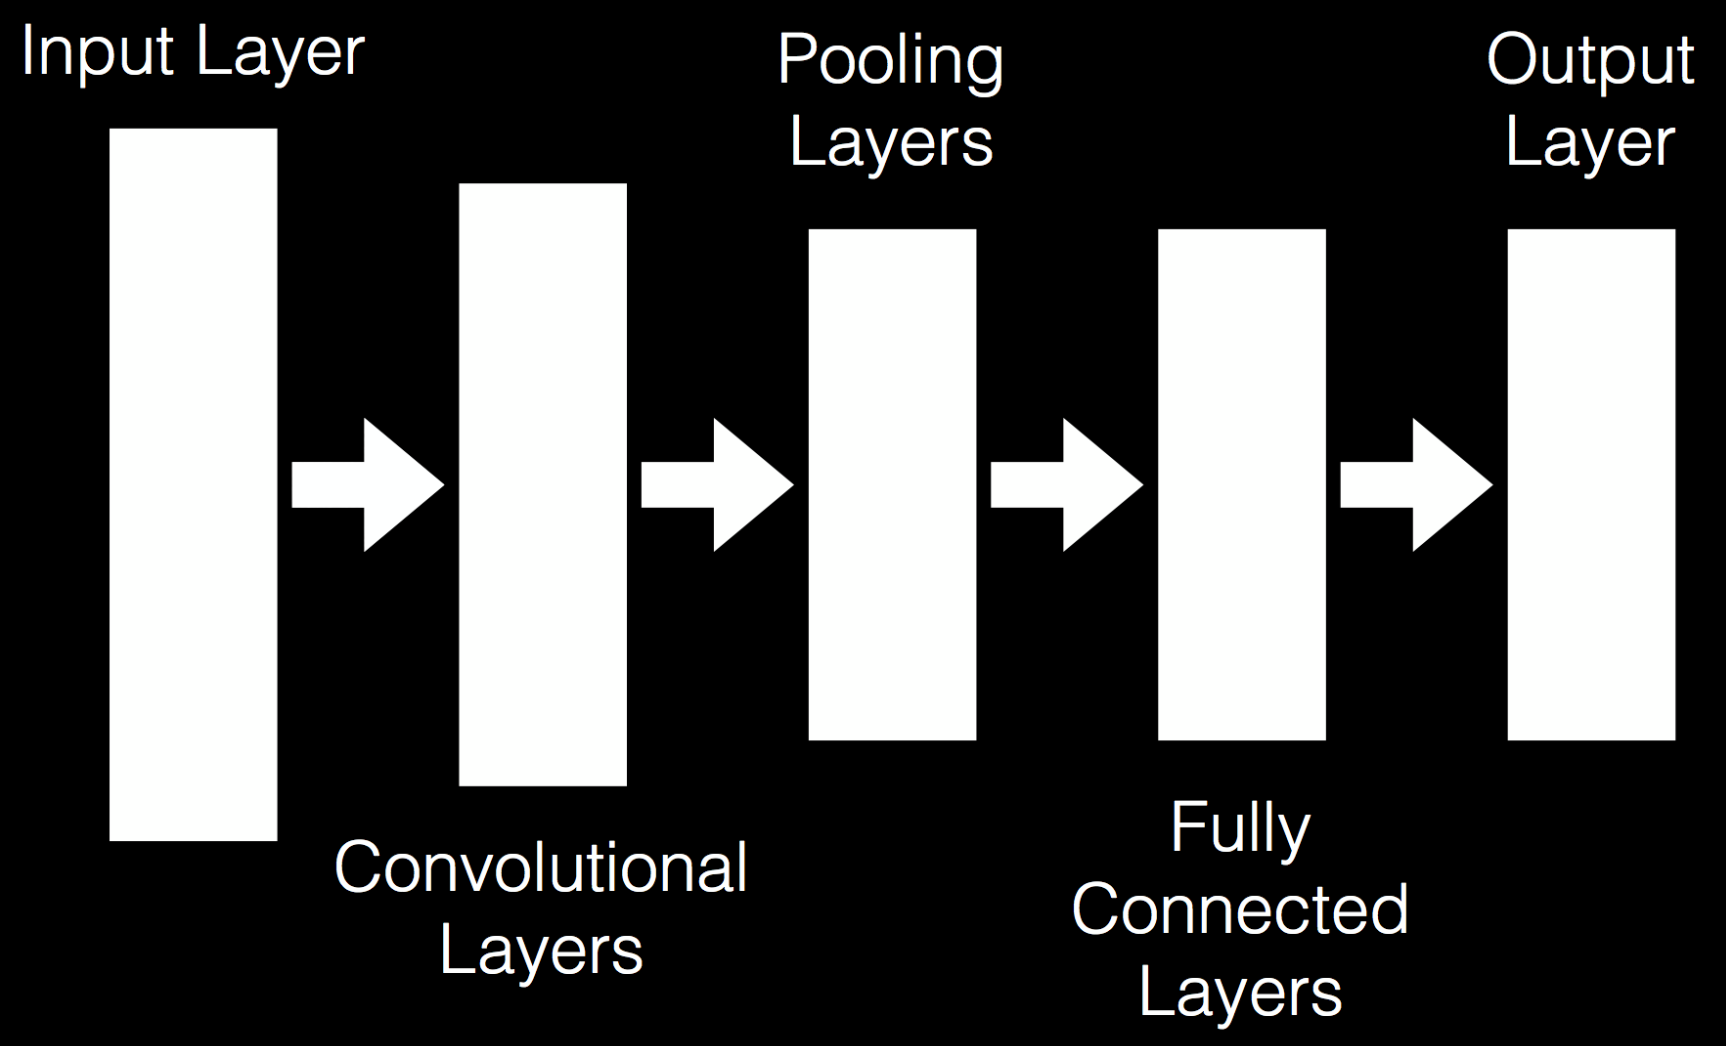
\includegraphics[width=3in]{stuff/convol5.png}}\\${}$\\${}$\\

There are three key features that make this CNN structure actually work: (1) local receptive fields, (2) shared weights,
and (3) pooling

\end{figure}

}








\frame
{
 \frametitle{1. Local Receptive Field}

\begin{figure}
\centering
\onslide<1>{{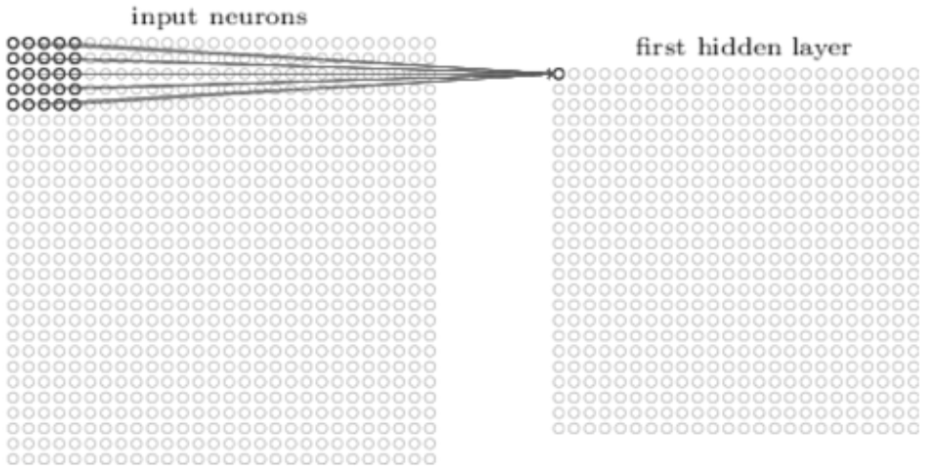
\includegraphics[height=2in]{stuff/convol6.png}}}
\end{figure}

\begin{itemize}
\item A group of pixes are a \emph{local receptive field}
\item Defined by the size of the kernel 
\item The image is transformed into the set of local receptive fields
\end{itemize}

}

\frame
{
 \frametitle{1. Local Receptive Field}

\begin{figure}
\centering
\onslide<1>{{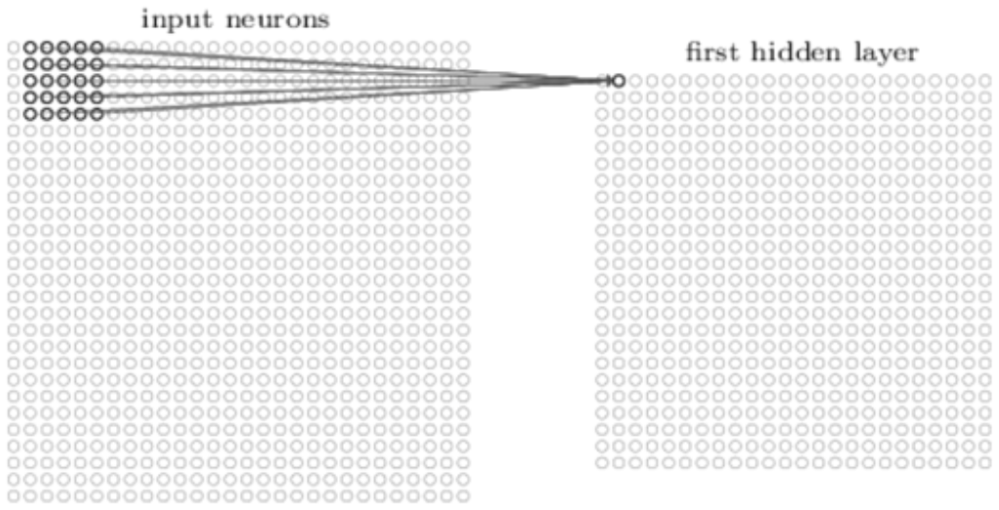
\includegraphics[height=2in]{stuff/convol7.png}}}
\end{figure}

\begin{itemize}
\item A group of pixes are a \emph{local receptive field}
\item Defined by the size of the kernel 
\item The image is transformed into the set of local receptive fields
\end{itemize}

}


\frame
{
 \frametitle{2. Shared Weights}

\begin{figure}
\centering
{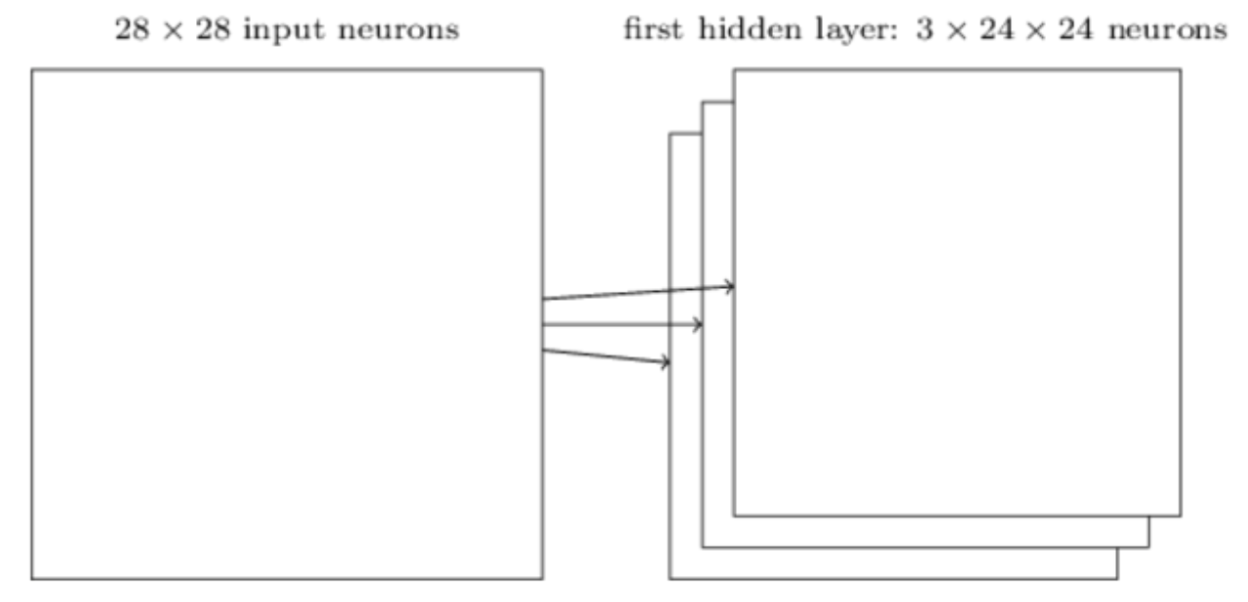
\includegraphics[height=2in]{stuff/convol8.png}}
\end{figure}

\begin{itemize}
\item Multiple convolutions are learned/used
\item Weights within a convolution are (obviously) shared
\end{itemize}

}


\frame
{
 \frametitle{3. Pooling}

\begin{figure}
\centering
{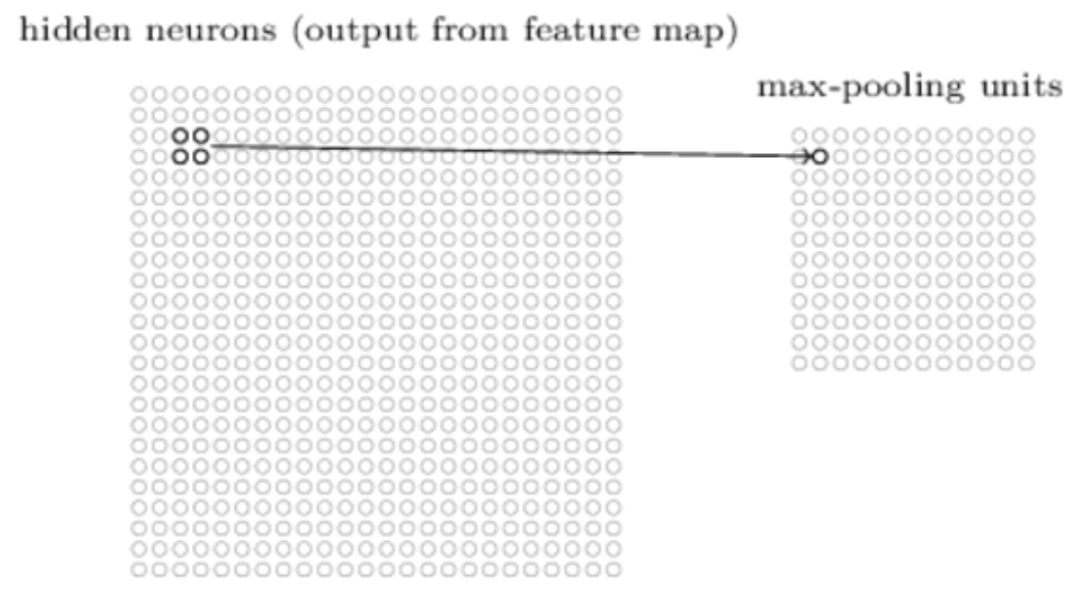
\includegraphics[height=2in]{stuff/convol9.png}}
\end{figure}

\begin{itemize}
\item Convolutional layers are simplified using, e.g., \emph{max pooling} 
\item This reduces computational complexity in downstream layers
\item In addition it provides a form of translational invariance 
\end{itemize}

}


\frame
{
 \frametitle{Fully Connected and Output Layers}

\begin{figure}
\centering
\fbox{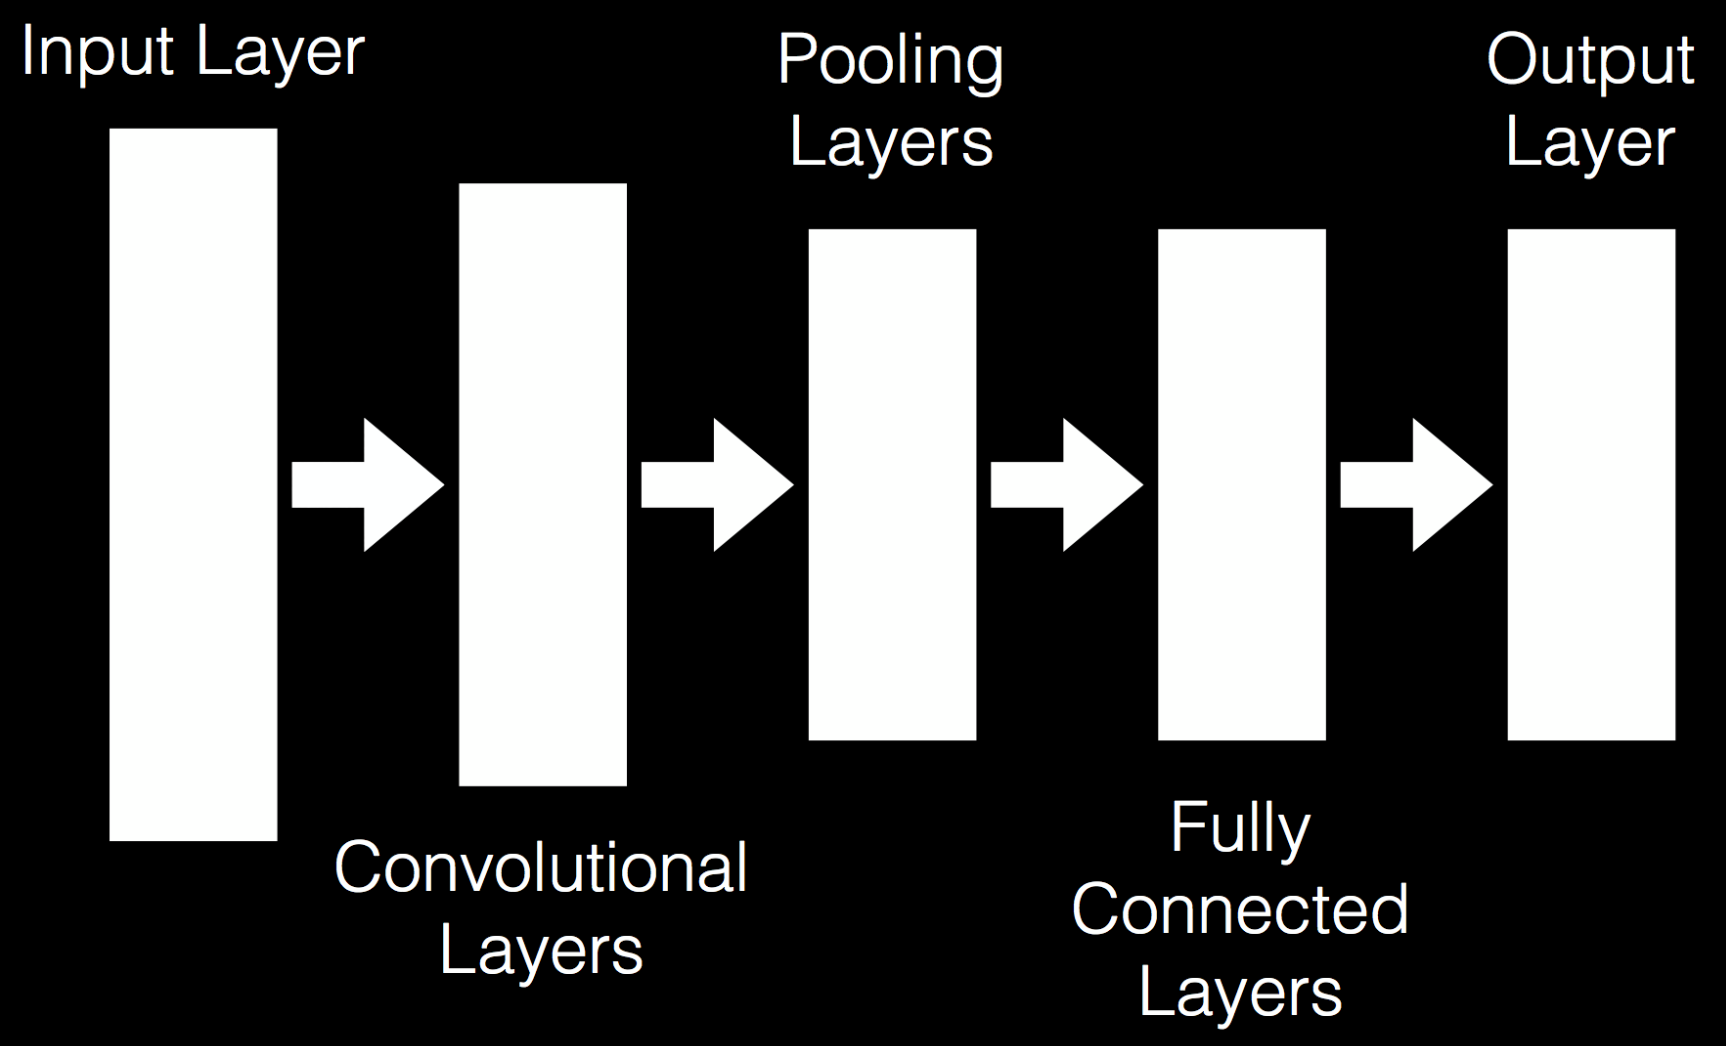
\includegraphics[width=2.5in]{stuff/convol5.png}}
\end{figure}

\begin{itemize}
\item Fully connected layers hierarchically aggregate learned features\\
\textcolor{gray}{-- they produces higher order features in standard NN manner} 
\item Softmax can be applied to the output layer $\eta_k, k=1, \cdots K$ 
to estimate the one-versus-all class probabilities of $K$ classes: 
$$ \frac{e^{\eta_k}}{\sum_{k'=1}^K e^{\eta_{k'}}}$$
\end{itemize}

}

\frame
{
 \frametitle{So a final CNN might look something like this...}

\begin{figure}
\centering
{\includegraphics[width=4in]{stuff/convol4.png}}
\end{figure}

}

\frame
{
\frametitle{Recurrent Neural Network (RNN)}

\begin{itemize}
\item A RNN is a NN where a hidden layer feeds back into itself
\item This allows the NN to exhibit dynamic temporal behavior
\item RNN's provide ``internal memory'' for sequence processing
\item They are very applicable to handwriting/speech recognition
\end{itemize}

\begin{figure}
\centering
\url{https://github.com/SirDudeness/BassGenerator}
\end{figure}
}

\frame
{
 \frametitle{Mores}

\url{github.com/sallamander/neural-networks-intro}\\
\textcolor{gray}{[Provides introductions in NumPy, Theano, Tensorflow, \& Keras]}\\
\url{neuralnetworksanddeeplearning.com} \textcolor{gray}{[General introduction]}\\
\url{cs231n.github.io/} \textcolor{gray}{[Convolution NN's for visual recognition]}\\
\url{deeplearning.net/tutorial/lenet.html} \textcolor{gray}{[Mathematics]}\\
\url{arxiv.org/abs/1503.02531} \textcolor{gray}{[Interpretation detractions]}\\
\textcolor{gray}{[Projects]}\\
\url{lasagne.readthedocs.org/en/latest/index.html}\\
(also, see nolearn for an scikit learn type of interface)\\
\url{cbinsignts.com/blog/python-tools-machine-learning}\\
\url{deeplearning.net/tutorial/lenet.html}\\
\url{deeplearning4j.org}\\
\url{caffe.berkeleyvision.org}\\
\textcolor{gray}{``How does deep learning work and how is it different from normal neural net works applied with SVM'' on quora.com differentiates deep learning from other methods.  Hinton's 2007 Google talk ``The Next Generation of Neural Networks'' introduces deep learning }

}

\frame
{
 \frametitle{Fine}
\begin{figure}
\centering
NN's \underline{do not} \textbf{currently} make machine learning any \emph{easier}...
\end{figure}
 
}

\end{document}
% autoencoders
% multilayer perceptron
% 




\frame
{
 \frametitle{How \emph{might} computers be able to do this?}
 
\Huge

 \begin{itemize}
\item<2-> Compress data
\item<2-> Keep the search simple
\item<2-> Segment image into objects
 \end{itemize}

}

\frame
{
 \frametitle{Image processing \emph{tasks}}

\begin{itemize}
\item Image processing libraries 
 \begin{itemize}
\item Scikit-image (skimage)
\item OpenCV (and dependencies) 
\item Python Imaging Library
\item Pillow (a fork of the above)
\item etc. 
 \end{itemize}
\end{itemize} 
}


\frame
{
 \frametitle{Image processing \emph{tasks}}
 
 
\begin{itemize}
\item Read

\onslide<2->{./dog\_cat  \\./dog\_cat/dog $\;$  ./dog\_cat/cat \\
\begin{figure}
\centering
\LARGE
$\bigg[\bigg[$\raisebox{-.9em}{\includegraphics[height=.5in]{dog1.jpg}$,$} \raisebox{-.9em}{\includegraphics[height=.5in]{dog2.jpg}$,$} \raisebox{-.9em}{\includegraphics[height=.5in]{dog3.jpg}}$\bigg]_,$\\
$\bigg[$\raisebox{-.9em}{\includegraphics[height=.5in]{cat1.jpg}$,$} \raisebox{-.9em}{\includegraphics[height=.5in]{cat2.jpg}$,$} \raisebox{-.9em}{\includegraphics[height=.5in]{cat3.jpg}}$\bigg]\bigg]$
\end{figure}
}
\normalsize

\item[] 
 \end{itemize}

}




\frame
{
 \frametitle{A first NN}
 
 We observe feature $X$.  Subsequently, we observe an associated continuous valued $Y$.
 Similar $X$'s seem to produce similar $Y$'s.  \\${}$\\

\underline{We want to ``understand'' what $Y$ will be upon observing $X=x$.}  \\${}$\\
 
 Let's design an NN with a node $\eta$ that captures the ``idea'' of $Y|X$
 This will be gauged by the NN's ability to predict Y $(\hat Y)$  from $X$.
 \textcolor{gray}{We will use a linear (i.e., identity) activation function to produce $\hat Y$}\\${}$\\
 
\onslide<2->{\hspace{1.75in}\xymatrix{
1 \ar[r]|{\beta_0}& \overset{\textcolor{gray}{(\hat Y)}}{\left\{ \eta \right\}} \\
X \ar[ur]|{\beta_1} &  \\
}}

${}$\\
\onslide<3->{We'll train the NN with a squared loss cost function $\frac{1}{2}\sum(Y_i-\hat Y_i)^2$}
}
\frame
{
 \frametitle{A second NN}
 
 We observe feature $X$.  Subsequently, we observe an associated binary outcome $Y$.
The outcomes $Y$ seem to be associated with $X$. \\${}$\\

\underline{We want to ``understand'' what $Y$ will be upon observing $X=x$.}  \\${}$\\
 
 Let's design an NN with a node $\eta$ capturing the ``idea'' of $\Pr(Y|X)$
 This will be gauged by the NN's ability to predict Y $(\hat p)$  from $X$.
 \textcolor{gray}{We will use a logistic (sigmoid) activation function to produce $\hat p$}\\${}$\\
 
\onslide<2->{\hspace{1.75in}\xymatrix{
1 \ar[r]|{\beta_0}&\overset{\textcolor{gray}{(\hat p)}}{\left\{ \eta \right\}}   \\
X \ar[ur]|{\beta_1} & \\
}}

${}$\\
\onslide<3->{We'll train the NN using the log loss cost function, $-\log L(\hat {\boldsymbol Y}|{\boldsymbol Y})$}
 
}



\frame
{
 \frametitle{A general approach to fitting NN's}
\begin{itemize}
\item[] NN's can be fit using gradient decent
\item<2-> \emph{Forward propagation} generates NN states from input features 
\item<3-> \emph{Backward propagation} is gradient decent on NN cost functions 
\item<4->[] \textcolor{gray}{Why is is it called \emph{backpropagation}? }
\item<5->[] \textcolor{gray}{[linear regression/af with squared loss cost function]}
\end{itemize}
\vspace{-.5em}
\onslide<6->{
\footnotesize
\begin{align*}
{} & -\frac{\partial}{\partial W_{j}^{(3)}}\frac{1}{2}\left(Y - \left(X^TW^{(0)}\right)W^{(1)}\right)^2 \\
= {} & -\frac{\partial}{\partial W_j^{(3)}} g_2\left(g_1\left(W^{(0)}\right)\right)
=  - \frac{\partial }{\partial g_1\left(W^{(0)}\right)} \frac{\partial g_1\left(W^{(0)}\right)}{\partial W_{j}^{(2)}} g_2\left(g_1\left(W^{(0)}\right)\right)\\
= {} & \textcolor{red}{\left(Y - \left(X^TW^{(0)}\right)W^{(1)}\right)} \textcolor{blue}{X^T W_j^{(2)} } =  
 \textcolor{red}{error}\times\textcolor{blue}{culpability} 
\end{align*}}
\vspace{-.25em}
\onslide<7->{
\footnotesize
\begin{align*}
{} & -\frac{\partial}{\partial W_{ij}^{(2)}}\frac{1}{2}\left(Y - \left(X^TW^{(0)}\right)W^{(1)}\right)^2 
= -\frac{\partial}{\partial W^{(0)}} g_3\left(g_2\left(g_1\left(W^{(0)}\right)\right)\right)\\
= {} & -\frac{\partial }{\partial g_2\left(g_1\left(W^{(0)}\right)\right)} \frac{\partial g_2\left(g_1\left(W^{(0)}\right)\right)}{\partial g_1\left(W^{(0)}\right)} \frac{\partial g_1\left(W^{(0)}\right)}{\partial W_{ij}^{(2)}} g_3\left(g_2\left(g_1\left(W^{(0)}\right)\right)\right)\\
= {} & \textcolor{red}{\left(Y - \left(X^TW^{(0)}\right)W^{(1)}\right)} \textcolor{blue}{W_j^{(3)} X_i} =  
 \textcolor{red}{error}\times\textcolor{blue}{culpability} 
\end{align*}}

}






\frame
{
 \frametitle{Artificial Neural Network (NN) \textcolor{black}{High Level Summary} }

\begin{columns}
\begin{column}{.6\textwidth}
\begin{itemize}
%\item The linear model $X^T{W^{(0)}_1}$\\ maps features onto ${\mathbb R}$
%$$\left[ X_1, X_2, X_3 \right] \left[\begin{array}{ccc} w^{{(0)}_{11}} & w^{{(0)}_{12}} & w^{{(0)}_{13}} \\ w^{{(0)}_{21}} & w^{{(0)}_{22}} & w^{{(0)}_{23}} \\ w^{{(0)}_{31}} & w^{{(0)}_{32}} & w^{{(0)}_{33}} \\ \end{array}\right]$$
\item The (non-linear) activation functions maps, e.g., $X^T{w^{(0)}_1}$\\
\textcolor{gray}{$\Bigg($and then, e.g., $\left\{\eta^{(1)}\right\}^T{w^{(1)}_1}\Bigg)$}
\\ onto a set of action potentials 

\item<2-> Input samples are embedded into NN's 
as a set of (``on'' or ``off") activations 
encoding one of many possible NN states or ``thoughts''

%The set of (``on'' or ``off") states of these activations encode an input sample into the NN as one of its many possible states or ``thoughts''


\item<3-> The topology (size and number of layers) of the NN influences the number of ``ideas'' and level of cumulative abstraction applied
\item<4-> The $w's$ are trained to identify input patterns that should map to similar NN states and ``thoughts''... %how will it learn what similar x's are?
\end{itemize}
\end{column}
\begin{column}{.5\textwidth}

\vspace{.25em}
\xymatrix{
&&  \left\{\eta^{(2)}_1\right\}\\
X_{i1} \ar[dr]|{w^{{(0)}_{12}}} \ar[ddr]|>>>>>>{w^{{(0)}_{13}}} \ar[r]^{w^{{(0)}_{11}}}  & \left\{\eta^{(1)}_1\right\} \ar[ur]|{w^{{(1)}_{11}}} \ar[dr]|<<<<<<{w^{{(1)}_{13}}} \ar[ddr]|>>>>>>{w^{{(1)}_{14}}} \ar[dddr]|>>>>>>{w^{{(1)}_{15}}}  \ar[r]^{w^{{(1)}_{12}}}  & \left\{\eta^{(2)}_2\right\}  \\
X_{i2} \ar@{.}[r] \ar@{.}[dr] \ar@{.}[ur] & \left\{\eta^{(1)}_2\right\}  \ar@{.}[r] \ar@{.}[dr] \ar@{.}[ur]  \ar@{.}[ddr] \ar@{.}[uur]  &\left\{\eta^{(2)}_3\right\} \\
X_{i3} \ar@{.}[ur] \ar@{.}[uur] \ar@{.}[r] & \left\{\eta^{(1)}_3\right\}  \ar@{.}[r] \ar@{.}[dr] \ar@{.}[ur]  \ar@{.}[uuur] \ar@{.}[uur]  &\left\{\eta^{(2)}_4\right\}\\
&&  \left\{\eta^{(2)}_5\right\}\\
%& \text{Election} \ar[ur]^{\Pr(Wins|Awesome)}_{0.98} \ar[dr]^{0.02}_{\Pr(\cancel{Wins}|Awesome)} &\\
%& &  0.004 \\
%\text{Hillary} \ar[ddr]_{\Pr(\cancel{Awesome})}^{0.8} \ar[uur]^{\Pr(Awesome)}_{0.2}&\\
% & & 0.72 \\
%& \text{Election} \ar[ur]^{\Pr(Wins|\cancel{Awesome})}_{0.9}  \ar[dr]^{0.1}_{\Pr(\cancel{Wins}|\cancel{Awesome})}&\\
%&& 0.08 \\
}

\vspace{.25em}
\end{column}
\end{columns}

}

